%%%%%%%%%%%%%%%%%%%%%%%%PREAMBLE%%%%%%%%%%%%%%%%%%%==========================================================================
\documentclass[a4paper,11pt]{book}
\usepackage[left=4.5cm,right=4.5cm,top=2.5cm,bottom=2.5cm]{geometry}

%%%%%%%%%  Packages %%%%%%%%%%%%%%%%%%%%%%%%%%%%%%%%%%%%
\usepackage{amsmath, amsthm, amssymb,latexsym}
\usepackage{mathabx}
\usepackage{enumerate}
\usepackage{mathtools}
\usepackage{multicol}
\usepackage[utf8]{inputenc}
\usepackage[spanish]{babel} 
\usepackage{color}
\usepackage{hyperref}
\usepackage{graphicx}
\usepackage{colortbl}
\usepackage{subcaption}
\usepackage{mathrsfs} 
\usepackage{imakeidx}
\usepackage{enumitem} %%%\item\labe
\usepackage{soul}
\usepackage{empheq}

%%%%%%%%%%%%%%% Para comentarios en el texto bo
  
\usepackage{todonotes}
\usepackage{marginnote}
\let\marginpar\marginnote
\usepackage{verbdef}

\usepackage{cancel}

\usepackage{changes}

\definechangesauthor[name={Fer}, color=red]{Fer}

\makeatletter
\@namedef{Changes@AuthorColor}{green}
\colorlet{Changes@Color}{green}
\makeatother
 

%%%%%%%%%%%%%%  Theorems like environments %%%%%%%%%%%%%%%%%%
\theoremstyle{plain}
\newtheorem{thm}{Teorema}[chapter]
\newtheorem{lem}[thm]{Lema}
\newtheorem{prop}[thm]{Proposición}
\newtheorem{cor}[thm]{Corolario}
\newtheorem{defi}[thm]{Definición}
\newtheorem{propi}[thm]{Propiedad}

\theoremstyle{remark}
\newtheorem{obs}[thm]{Observación}

\newcounter{example}[section]
\newenvironment{example}[1][]{\refstepcounter{example}\par\medskip
   \noindent \textbf{Ejemplo~\theexample. #1} \rmfamily}{\medskip}
   
   
%===============LABEL ITEM =========================
\makeatletter
\newcommand{\labitem}[2]{%
\def\@itemlabel{#1}
\item
\def\@currentlabel{#1}\label{#2}}
\makeatother
\makeatletter
\def\namedlabel#1#2{\begingroup
    #2%
    \def\@currentlabel{#2}%
    \phantomsection\label{#1}\endgroup
}
\makeatother



%%%%%%%%%%%%%%%%% New commands %%%%%%%%%%%%%%%%%%%%%%%
\newcommand{\orlnor}{\|_{L^{\Phi}}}
\newcommand{\linf}{\|_{L^{\infty}}}
\newcommand{\lphi}{L^{\Phi}}
\newcommand{\lpsi}{L^{\Phi^{\star}}}
\newcommand{\wphi}{W^{1}\lphi}
\newcommand{\wphit}{W^{1}\lphi_T}
\newcommand{\wphittilde}{\widetilde{W^1}\lphi_T}
\newcommand{\sobnor}{\|_{W^{1}\lphi}}
\newcommand{\sobnort}{\|_{W^{1}\lphi_T}}
\newcommand{\rr}{\mathbb{R}}
\newcommand{\nn}{\mathbb{N}}
\DeclareMathOperator{\sign}{sign}
%%%%%%%%%%%%%%%%%%%
\DeclareMathOperator*{\sen}{sen}
\newcommand{\F}{\mathtt{F}}
\newcommand{\f}{\pmb{f}}
\newcommand{\V}{\operatorname{V}}
\newcommand{\Ves}{\operatorname{essV}}
%======================Document===========================================

\makeindex[columns=2, title=Glosario]

\makeindex[name=Simbolo,columns=3, title=Indice de Símbolos]



\begin{document}
\hyphenation{a-ni-so-tro-pic}

\numberwithin{equation}{section}

\title{Soluciones Periódicas a Ecuaciones con Medidas mediante el Método Shoothing.}
\author{ Fernando D. Mazzone. \thanks{SECyT-UNRC, FCEyN-UNLPam and CONICET.}\\
 Sonia E. Acinas. \thanks{ FCEyN-UNLPam and CONICET}\\
 Lorenzo F. Sierra. \thanks{ FCEyN-UNLPam.}\\
 \textcolor{blue}{Debe haber una formato para las tesis.}\\
 \textcolor{blue}{ Generalmente en la caràtula aparece el postulante}\\
 \textcolor{blue}{ y debajo los directores}\\
 
}
\date{}
%\thanks{Agradecimiento}


    \maketitle
%====================================================================
%\begin{abstract}
%Anotaciones y ejercicios del Capitulo I del Libro: Topological Methods in the Study of Bourdary Value Problems- Pablo Amster
%\end{abstract}

\begingroup%Locallizing the change to `thefootnote'.
\renewcommand{\thefootnote}{}%Removing the footnote symbol.
%\footnotetext{\textbf{2010  AMS Subject Classification.} Primary: 34C25 Secondary: 34B15}
%\footnotetext{\textbf{Keywords and phrases:} periodic solutions, Orlicz spaces, Euler-Lagrange equation, critical point}
\endgroup
\chapter*{}
%\pagenumbering{Roman}
%\setcounter{page}{3}
\begin{flushright}
\textit{Dedicatoria}
\end{flushright}

\chapter*{Agradecimientos}

{\color{green}
Sería bueno que agradezcas también a la UNLPam y  a la UNSL  por darte la oportunidad de realizar estudios de posgrado, a los profesores de la maestría, a la facultad por el financiamiento recibido por el proyecto. También podes agradecer a tus afectos, generalmente se dice ``por la paciencia que te tuvieron todos estos años'', en fin ....esto es personal tuyo pero es bueno recordar acordarse de todo lo que contribuyó al logro.v Por ahí me olvido de algo

}

En primer lugar quisiera agradecer al Dr. Fernando Mazzone y a la Dra. Sonia Acinas, por haberme guiado en la realización de esta tesis, por el tiempo dedicado, por su constante ayuda y paciencia. 

Al Cluster Tecnológico Río Cuarto por brindar acceso a “Dorotea”: un equipo de análisis de datos de última generación con una gran capacidad de procesamiento de cómputos, destinado a fomentar el desarrollo de modelos de IA.



\tableofcontents



\chapter{Introducción}
El objetivo de esta tesis es encontrar soluciones periódicas a ecuaciones diferenciales con medidas o MDE\index{MDE}, las cuales se pueden definir de manera general como 
\comment{Le cambiaría la función $F$ por la $f$ (hay una $F$ más abajo que no es la misma que la que aparece aca)}
\begin{equation*}
	\left\lbrace \begin{array}{l} \label{eq:problema A}
		d\varphi=F(t,\varphi(t))\;d \mu\\
		\varphi(0)-\varphi(T)=0,
	\end{array}\right. \tag{${MDE}$}
\end{equation*}
donde $F:[0,T]\times\rr^n\to\rr^{n\times m}$ es una función con valores matriciales, $\mu$ es una medida vectorial con valores en $\rr^m$, $\varphi:[0,T]\to \rr^n$ es una función de variación acotada  y $d\varphi$ es la medida vectorial Lebesgue-Stieltjes asociada a $\varphi$.

 Las MDE intervienen en modelos no suaves de varias ramas de la ciencia, como los modelos que describen el movimiento de moléculas en gases ideales hasta el análisis de la dinámica \highlight[comment={No quedará mejor expresado si decimos ``de los impactos de una pelota en una raqueta''? }]{de la pelota raqueta}. En  física e ingeniería mecánica intervienen en el estudio de materia granular y \reversemarginpar\highlight[comment={Qué son los motores de arena?. Lo googlie y me parece que son como filtros de pileta. No los denominaremos de otra forma en argentina?}]{ motores de arena}; en la robótica, se usan para estudiar impactos en las articulaciones (ver \cite{Brogliato} y \cite{ALeonov}). Un caso particular donde intervienen MDE es \replaced{aquel}{aquél} dado por los modelos impulsivos, ver \cite{Bainov},\cite{Bainov_2} y \cite{Lakshmikan}. Por ejemplo, en los sistemas mecánicos se puede pensar que el impacto entre dos cuerpos es un fenómeno de muy corta duración que implica un cambio brusco en la dinámica de los cuerpos. Es por eso que,\normalmarginpar\comment{Para mi no iría coma aquí} se suele representar \textcolor{red} {a}\comment{Está en rojo} los impactos como fuerzas muy grandes que actúan en un tiempo infinitamente corto. Supongamos que durante el impacto o colisión actúa una fuerza $F$ y que este ocurre en un intervalo $[t_0,t_0+\Delta t]$, entonces el cambio en la cantidad de movimiento es igual al impulso que genera la fuerza \index{impulso} \cite{Serway}, o sea
$$I=\Delta p=\int_{t_0}^{t_0+\Delta t}F(s)ds.$$
Si suponemos que la fuerza actúa\comment{Le buscaría un sinónimo a actúa, está muy repetido} en un intervalo muy chico, tanto que podemos decir que es instantánea, entonces el impulso es
    \begin{equation*}
        I=\lim_{\Delta t \to 0}\int_{t_0}^{t_0+\Delta t}F(s) ds. 
    \end{equation*}
    \newpage
Para que el impulso $I$ sea distinto de cero, $F(\cdot)$ debe tomar valores \highlight[comment={ No lo diría así, en realidad hacer infinito a $F$ tampoco arreglaría nada. ¿Qué te aparece decir lo siguiente? Si en la integral tuviesemos una función  integrada respecto a la medida de lebesgue el límite sería cero por la absoluta continuidad de la integral. Por eso necesitamos integrar respecto a medidas que no sean absolutamente continuas respecto a la medida de lebesgue}]{infinitos} ya que la medida de Lebesgue del intervalo tiende a cero. Por eso, es conveniente tomar a la fuerza como una medida de Dirac concentrada en el tiempo $t_0$ (la cual expresaremos como $\delta_{t_0}$\index[Simbolo]{$\delta_{t_0}$}) y de magnitud $I$, es decir $F(t)=I\delta_{t_0}$. A este tipo de fuerza se la  denomina fuerza impulsiva\index{fuerza impulsiva}.

{\color{green} Otra fuente de problemas con medidas son los problemas de control. Podes agregar una breve mención sobre eso (podes sacar una idea del primer párrafo en el prefacio de \cite{S.T.Zavalishchin}). También agregaría algo asi: <<Más allá de las aplicaciones, los problemas de ecuaciones diferenciales con medidas son, desde el punto de vista exclusivamente matemático, una generalización natural de las ecuaciones diferenciales ordinarias y a nuestro juicio este hecho ya justificaría su estudio. Varias teorías de integración han sido utilizadas para abordar problemas como los planteados en esta tesis, a saber integrales de Lebesgue-Stieltjes, Perron-Stieltjes, Kurzweil-Henstock (ver por ejemplo    \cite{S.Schwabik320,JaroslavKurzweil1411,StefanSchwabik75,EveraldoM.Bonotto420}).>>}


\begin{example} \label{ejemplo1}
    Supongamos que un cuerpo de masa $m$ se mueve con velocidad constante sobre una recta, y se somete a impulsos $I_k$ en los instantes $t_k$. Como el impulso es el cambio en la cantidad de movimiento (\cite{Serway}), entonces $I_k=mv(t_k^+)-mv(t_k^-)$. Podemos decir que si el movimiento del cuerpo está dado por la función $x(t)$, entonces cumple la siguiente ecuación 
    \begin{equation}
	\left\lbrace \begin{array}{lll} 
		\label{eq:imp}
        x''(t)=0 & \text{si }& t\neq t_k,\\
		x'(t_k^+)-x'(t_k^-)=\dfrac{I_k} {m} & \text{ para }& k=1,..,r.\tag{${PI}$}
	\end{array}\right. 
\end{equation}
Si ahora consideramos la fuerza impulsiva $F(t)=\displaystyle\sum_{k=1}^r I_k\delta_{t_k},$ entonces podemos \deleted{puedo} escribir el problema impulsivo \ref{eq:imp} como una \ref{eq:problema A}
$$d(x'(t))=\sum_{k=1}^r\dfrac{I_k}{m}\delta_{t_k}\textrm{\todo{No escribiría $d(x'(t))$ porque reigurosamente hablando sería el diferencial de una constante, sería $0$. Pondría simplemente $dx'$ (fijate que en el miembro de la derecha no hay $t$, tampoco te hace falta a la izquierda}}$$
\end{example}
\textcolor{blue}{
Los modelos impulsivos intervienen en otras ciencias, además de física o matemática, como por ejemplo en biología.}
 

\begin{example}\label{ejemplo2}
\textcolor{blue}{La ecuación 
\begin{equation}\label{ec:biomasa}
    x'=rx\left(1-\dfrac{x}{K}\right),
\end{equation}
describe los cambios en el número de individuos $x(t)$ en una población aislada, de alguna especie biológica con una taza de reproducción $r$, en un ambiente estacionario con una capacidad máxima de $K$. Para ser más precisos, supondremos que $x(t)$ es la cantidad de biomasa de una determinada especie de microorganismo cultivado en un biorreactor. Los efectos externos sobre el desarrollo de la especie pueden provocar saltos en la cantidad de biomasa $x(t)$. Esto es posible, por ejemplo, con una sola extracción de una parte de la biomasa o con la introducción de una cantidad adicional de biomasa. Los  efectos externos en el momento $t=t_k$ generan que la  cantidad de biomasa sufra un incremento, es decir 
$$I_k=\Delta x(t_k)=x(t_k^+)-x(t_k^-).$$
Como en el ejemplo anterior, este tipo de problemas puede ser descripto usando MDE.
En este caso, tendríamos una parte de la ecuación no impulsiva o suave $f(t,x)=rx\left(1-\dfrac{x}{K}\right)$, en donde actuaría la medida de Lebesgue (usaremos el símbolo $d\lambda$, para diferenciarla de otras medidas\comment{ya está dicho}) y otra parte impulsiva o no suave donde estaría el impulso $I_k$ con la medida de Dirac.
\begin{equation*}
    d(x)=rx\left(1-\dfrac{x}{K}\right)d\lambda +g(x)d\delta_{t_k}.
\end{equation*}}
\end{example}



%\begin{example}
%    \begin{equation*}
%	\left\lbrace \begin{array}{lcr} 
%		x'=1+x^2,\\
%        x(0)=0\\
%		\Delta x(t_k)=-1 &t_k=\frac{k\pi}{4}&k=1,2,....
%	\end{array}\right. 
%\end{equation*}
%Si notamos $d\lambda$ a la medida de Lebesgue \index[Simbolo]{$d\lambda$}, el problema anterior se puede expresar como una MDE de la siguiente manera
%\begin{equation*}
%	\left\lbrace \begin{array}{lcr} 
%		x'=1+x^2 \;d\lambda-\displaystyle\sum_{k=1}^{\infty}d\delta_{t_k}(t),\\
%        x(0)=0.\\
	%	\end{array}\right. 
%\end{equation*}
%La solución es $x(t)=\tan(t-\frac{k\pi}{4})$ donde $\frac{k\pi}{4}\leq %t <\frac{(k+1)\pi}{4}$, y tiene período $\pi/4$.
%\begin{figure}[h!]
%    \centering
%    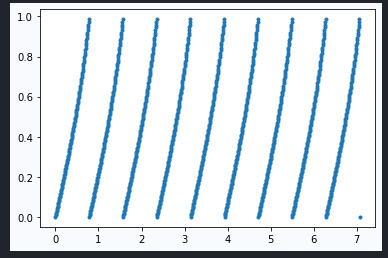
\includegraphics[width=0.7\linewidth]{img.ejem1.png}
%    \caption{}
%    \label{fig:ejemple1}
%\end{figure}



%\end{example}

Las ecuaciones impulsivas se pueden generalizar para casos donde actúan fuerzas no impulsivas $f(t,x)$ y/o  donde se aplique una cantidad infinita de impulso. Un caso general se puede ver en \cite{Bainov}, está dado por
	\begin{equation*}
		\left\lbrace \begin{array}{l}
			x''=f(t,x(t)) \; \text{si }\; t\neq t_k\\
			 x'(t_k^+)-x'(t_k^-)=I_k \; \text{ donde }\; k=1,2,....,
		\end{array}\right. 
	\end{equation*}
donde, como vimos en el ejemplo \ref{ejemplo1}, se pude pensar a los impulsos como suma de deltas de Dirac concentradas en $t_k$ y 
empleando la medida de Lebesgue $d\lambda$.\index[Simbolo]{$d\lambda$}
$$dx'=f(t,x(t)) d\lambda +\sum_{k=1}^{\infty}I_k\;d\delta_{t_k}$$

Para resolver ecuaciones como \eqref{eq:problema A}, usaremos una 
metodología inspirada 
en   la sección 1.3 del
libro de Pablo Amster.
Allí utiliza el método Shooting para hallar soluciones al problema de contorno periódico 

	\begin{equation*}
		\left\lbrace \begin{array}{l}
			u'=f(t,u(t))\\
			u(0)-u(T)=0,
		\end{array}\right. 
	\end{equation*}
donde $f$ es una función continua y Lipschitz en la segunda variable $u\in\rr^2$.  La idea que propone Pablo Amster \replaced{consiste}{conciste} en buscar una solución $u_\alpha$ al problema de valores iniciales 
	\begin{equation*}
	\left\lbrace \begin{array}{lcl}
		u'&=&f(t,u(t))\\
		u(0)&=&\alpha,
	\end{array}\right. 
\end{equation*}
y buscar un valor de $\alpha\in\rr^2$ tal que $u_\lambda(T)=\alpha$. Es decir,
$u_\alpha$ no es otra cosa que  un punto fijo del operador de Poíncare\index{operador de Poíncare} $P:\rr^2\to \rr^2$, definido como $P(\alpha)=u_\alpha(T)$. Bajo ciertas condiciones, aplicando el Teorema de Brouwer \cite{Amster} al operador podemos asegurar la existencia de la solución al problema periódico. 

En el capítulo 2 haremos una breve introducción a la medida de Lebesgue-Stieltjes y sus propiedades. 
En el capitulo 3 se encuentran los resultados principales de este trabajo de tesis. En la sección 3.1 vamos a ver como transformar el problema \eqref{eq:problema A} con medidas vectoriales a uno donde intervenga una sola medida positiva. En la sección 3.2 estableceremos las condiciones para la existencia de soluciones al problema de valores iniciales y su continuación a intervalos máximos. En la sección 3.3 enunciaremos y demostraremos una versión del teorema de Gronwall que hemos obtenido para medidas de Borel. A partir de este teorema, probaremos  la continuidad del operador de Poincaré y finalmente podremos usar el Teorema Brouwer y 
hallar un punto fijo para el operador de Poincaré.  











% 
 \chapter{Medida de Lebesgue-Stieltjes}




En este trabajo denotaremos por $\rr$ al conjunto de todos los números reales y por $\rr^n$ al conjunto de todas las $n$-uplas con componentes reales.  Si $x\in \rr^n$, escribiremos la norma euclídea como $|x|=\sqrt{x_1^2+\cdots x_n^2}$\index[Simbolo]{$\vert x\vert$}, y otra norma que usaremos será la del caminante  $|x|_1=|x_1|+\cdots +|x_n|$. \index[Simbolo]{$\vert x\vert_1 $}  
El producto interno que usaremos es el  usual en $\rr^n $, definido por  $x\cdot y=x_1y_1 + \cdots+
x_ny_n$. Se puede pensar al vector $x$ como una matriz de $n\times 1$, y notaremos con $x^*$ \index[Simbolo]{$x^*$}a la matriz traspuesta $1\times n$ de $x$.

\textcolor{blue}{El conjunto de todas las funciones continuas, $f:[0,T]\to \rr^n$ será denotado como $C([0,T],\rr^n)$ o simplemente $C([0,T])$\index[Simbolo]{$C([0,T])$} si su codominio es $\rr$.    Escribiremos $f'(x)$ para la derivada de funciones escalares como para funciones de $\rr$ a $\rr^n$. }

Sea $\mathcal{X}$ un espacio topológico. Se define \added{la }  $\sigma$-álgebra  de Borel\index{$\sigma$-álgebra} \replaced{como }{a} la $\sigma$-álgebra generada por los conjuntos abiertos de $\mathcal{X}$, y la  denotaremos $\mathscr{B}(\mathcal{X})$. \index[Simbolo]{$\mathscr{B}(\mathcal{X})$}
En particular, $\mathscr{B}(\rr)$ \index[Simbolo]{$\mathscr{B}(\rr)$}será la $\sigma$-álgebra generada por los intervalos abiertos de $\rr$ y $\mathscr{B}([a,b])$\index[Simbolo]{$\mathscr{B}([a,b])$} la generada por los intervalos abiertos relativos de $[a,b]$. Diremos que una medida es de Borel si esta definida sobre \added{la } $\sigma$-álgebra de Borel.\index{$\sigma$-álgebra!Borel} \comment{Pondría en otro lado esta notación de diferencia de conjuntos} Dados dos conjuntos $A$ y $B$, notaremos $A\setminus B$\index[Simbolo]{$A\setminus B$} al complemento de $B$ respecto de $A$.




\section{Funciones de variación acotada}
\textcolor{blue}{Cuando definimos \ref{eq:problema A} dijimos que $\varphi$ era una función de variación acotada y que entendíamos a  $d\varphi$ como la medida de Lebesgue-Stieltjes de $\varphi$. En esta sección daremos las definiciones y principales resultados, que nos permitan definir la medida de Lebesgue-Stieltjes de una función de variación acotada.}

\begin{defi}
	Dada $u:[0,T]\to \rr$\comment{En esta y las definiciones de abajo, no vamos a necesitar funciones con valores a $\rr^n$?}, definimos la variación \index{variación!} de $u$ como \index[Simbolo]{$\V(u,[0,T])$}\label{def:variación}
	$$\V(u,[0,T])=\sup_{\substack{ t_i\in [0,T]\\
			0\leq\reversemarginpar \textrm{\todo{Pondría $0=t_1$ y $t_n=T$ y debajo del supremo solo el símbolo de la partición $P$}}t_1 < t_2< \dots < t_n  \leq T}}\left\lbrace \sum_{i=1}^{n-1}|u(t_{i+1})-u(t_i)|\right\rbrace $$
\added{donde el supremo se toma sobre todas las particiones $P=\{t_1,\ldots,t_n\}$ del intervalo $[0,T]$} 
\end{defi}

\begin{defi}
\textcolor{blue}{ Una función $u:[0,T]\to \rr$ es de variación acotada\index{variación!acotada} en el intervalo $[0,T]$ si $\V(u,[0,T])<\infty$.
	El conjunto de todas las funciones de variación acotada en $[0,T]$ se denota como $BV([0,T],\rr)$.\index[Simbolo]{$BV([0,T],\rr)$} Si además $u(0)=\alpha$ diremos que $u\in BV_\alpha([0,T],\rr^n)$. \index[Simbolo]{$BV_\alpha([0,T],\rr^n)$}}
	%Si además $u(0)=u(T)$ entonces diremos que $u\in BV_T([0,T],\rr)$. \index[Simbolo]{$BV_T([0,T],\rr)$}
\end{defi}
\begin{lem} \label{lem:var-acotada}
    \textcolor{blue}{ $u\in BV_\alpha([0,T],\rr^n)$, entonces para todo $t\in[0,T]$ existe $K>0$ tal que $|u(t)|\leq K$.  }
\end{lem}
\begin{proof}[Dem.]\textcolor{blue}{
Si $u\in BV_\alpha([0,T],\rr^n)$, entonces
    \begin{equation}
        |u(t)|\leq |u(t)-u(0)|+|\alpha|\leq V(u,[0,t])+|\alpha|\leq V(u,[0,T])+|\alpha|.
    \end{equation}
Luego llamando $K=V(u,[0,T])+|\alpha|$, tenemos que $|u(t)|\leq K$.  }
    
\end{proof}


    
\begin{prop}\textcolor{blue}{ \label{pro:completo}
     Si $d(u,v)=V(u-v,[0,T])$ \index[Simbolo]{$d$}, entonces $\left(BV_\alpha([0,T],\rr^n),d\right)$ es un espacio métrico completo.}
\end{prop}
\begin{proof}[Dem.]
    \textcolor{blue}{Para que $\left(BV_\alpha([0,T],\rr^n),d\right)$ sea un espacio métrico la función $d$ tiene que ser una métrica. Sean $u,v,w\in BV_\alpha([0,T]$:
\begin{itemize}
\item Si $d(u,v)=0$ entonces $V(u-v,[0,T])=0$, por lo tanto $v-u$ es constante y como $u(0)=v(0)$ resulta que $u=v$. 
\item $d(u,u)=V(u-u,[0,T])=0$. \comment{Me parece que este  y el inciso que sigue son redundantes, porque el primero de todos era un si y solo si}
\item $d(u,v)=V(u-v,[0,T])>|u(0)-v(0)-u(T)+v(T)|>0$.
\item Usando la definición de variación \ref{def:variación}
\begin{equation*}
    \begin{split}
    d(u,v)&=\sup_{\substack{ t_i\in [0,T]\\
0\leq t_1 < t_2< \dots < t_n  \leq T}}\left\lbrace \sum_{i=1}^{n-1}|u(t_{i+1})-v(t_{i+1})-u(t_i)+v(t_{i})|\right\rbrace\\&=
\sup_{\substack{ t_i\in [0,T]\\
0\leq t_1 < t_2< \dots < t_n  \leq T}}\left\lbrace \sum_{i=1}^{n-1}|v(t_{i+1})-u(t_{i+1})-v(t_i)+u(t_{i})|\right\rbrace\\&=d(v,u).
    \end{split}
\end{equation*}
\item Sea $0=t_1,t_2,\ldots t_k=T$ una partición del intervalo $[0,T]$, entonces
\begin{equation*}
    \begin{split}
        |u(t_{i+1})-v(t_{i+1})-u(t_i)+v(t_{i})|&   \leq |u(t_{i+1})-w(t_{i+1})-u(t_i)+w(t_{i})|\\&+ |w(t_{i+1})-v(t_{i+1})-w(t_i)+v(t_{i})|,
    \end{split}
\end{equation*}
sumando para $i=1$ hasta $k-1$ y tomando supremo sobre todas las particiones del intervalo $[0,T]$ tenemos que 
$$V(u-v,[0,T])\leq V(u-w,[0,T])+V(w-v,[0,T]).$$
Por lo tanto $d(u,v)\leq d(u,w)+d(w,v)$.
    \end{itemize}
Veamos que $\left(BV_\alpha([0,T],\rr^n),d\right)$ es completo. Sea $\{u_n\}$ una sucesión de Cauchy\replaced{. Como toda sucesión de Cauchy es acotada,}{,   luego} existe una constante $K$ tal que $\forall n$ $d(u_n,0)=V(u_n,[0,T])\leq K$. Además por \added{Lema } \ref{lem:var-acotada} para cualquier $t\in[0,T]$
\begin{equation} \label{eq:desigualdad d}
|u_n(t)|\leq|u_n(t)-u_n(0)|+|u_n(0)|\leq V(u_n,[0,T])+|\alpha|\leq K.
\end{equation}
Luego por el \replaced{Primer Teorema de Helly}{teorema de Helly's} \replaced{(ver \cite{Natanson})}{\cite{Natanson}}
\comment{Va a quedar mejor si identificas con más presisión el teorema}
existe una \replaced{subsucesión}{subsecesión} convergente\replaced{. Una sucesión de Cauchy que posee una subsucesión convergente es, en si misma, convergente. Por}{, y por} lo tanto la sucesión es convergente.
}
\end{proof}







El siguiente resultado permite caracterizar a las funciones de variación acotada.

\begin{thm}\label{T-VB}
	 $u\in BV([0,T],\rr)$ si y sólo si $u$ se puede escribir como la diferencia de dos funciones crecientes en $[0,T]$.
\end{thm}

La demostración de este teorema y más información sobre funciones de variación acotada puede encontrarse en \cite{Carter}. %(Teorema  2.7.2). 
\begin{cor}
	Si $u\in BV([0,T],\rr)$, entonces 
	\begin{itemize}
		\item para $0<t<T$ los siguientes límites existen y son finitos
		$$u(t^+)=\lim\limits_{s\to t^+}u(s) \ \ \ \ u(t^-)=\lim\limits_{s\to t^-}u(s);$$\index[Simbolo]{$u(t^+)$}
		\item $u(0^+)$ y $u(T^-)$ existen y son finitos.
	\end{itemize}
\end{cor}






\section{Medida de Lebesgue-Stieltjes}
A continuación, vamos a enumerar algunos resultados necesarios para definir la medida de Lebesgue-Stieljes asociada a una función de variación acotada. Para un desarrollo mas detallado ver \cite{folland}.
\subsection{Medida de Lebesgue-Stieltjes en $\mathbb{R}$}
 
Vamos a definir la medida de Labesgue-Stieltjes para una función \replaced{no decreciente}{de creciente}\comment{El creciente que debería sustiuirse por no decreciente aparece un montón de veces, no te lo voy a corregir cada vez} y continua a izquierda. El mismo desarrollo se puede hacer para funciones \replaced{no crecientes}{decrecientes}, con la salvedad de que la medida generada \replaced{es}{en} negativa.


\begin{defi}\label{def:premedida}
Sea $\mathcal{A}$ un álgebra\added{ de subconjuntos de $X$, es decir $\mathcal{A}$ es cerrado para uniones e intersecciones finitas y $\emptyset,X\in\mathcal{A}$}. Diremos que la función $\mu_0:\mathcal{A}\to [0,\infty)$ es una premedida\index{premedida}, si cumple 
 
 
\begin{itemize}
    \item $\mu_0(\emptyset)=0,$
    \item si $\displaystyle\left\{A_i\right\}_1^\infty$ es una familia de conjuntos disjuntos tal que $\displaystyle\bigcup_1^\infty A_i\in \mathcal{A}$, entonces $\displaystyle\mu_0\left(\bigcup_1^\infty A_i\right)\leq \sum_1^\infty \mu_0\left(A_i\right).$ 
\end{itemize}

\end{defi}
\textcolor{blue}{Vamos a notar con $\mathcal{A}$ \index[Simbolo]{$\mathcal{A}$} a la colección de todos los conjuntos que se escriben como unión finita de intervalos disjuntos de la forma $[a,b)$ con $-\infty<a<b<\infty$, más el conjunto $\emptyset$. En proposición 1.2 y  1.7 de \cite{folland} se muestra que  $\mathcal{A}$ es un álgebra y que además genera la $\sigma$-álgebra de Borel.}

%\begin{prop}El conjunto $\mathcal{A}$ cumple que:
%\label{prop:algebra de borel}
%	\begin{itemize}
%		\item $\mathcal{A}$ es un álgebra.\index{álgebra}
%		\item La $\sigma$-álgebra generada por $\mathcal{A}$ es la $\sigma$-álgebra de Borel, ($\mathscr{B}(\rr)$).\index{$\sigma$-álgebra}\index[Simbolo]{$\mathscr{B}(\rr)$}
%	\end{itemize}
%\end{prop}


Sea  $u:\rr \to \rr$  creciente y continua a izquierda y sean  $[a_j,b_j)$ intervalos disjuntos para $j=1, \cdots ,m$. Por la proposición 1.15 de \cite{folland}, la función  $\mu_{0}$ definida como 

$$\mu_{0}\left( \bigcup_{j=1}^m[a_j,b_j)\right)  =\sum_{j=1}^{m}\left(u(b_j)-u(a_j)\right) $$\index[Simbolo]{$\mu_{0}$}
es una premedida  en $\mathcal{A}$. A partir de una premedida podemos definir  medida exterior para cualquier conjunto arbitrario $E\subset\rr$ \index{medida! exterior} de la siguiente manera 
$$\mu^{*}(E)=\inf\left\lbrace \sum_{ j=1 }^{\infty}\mu_{0}(A_j) \mid \ A_j\in \mathcal{A}, \ \  E\subset\bigcup_{j=1}^{\infty}A_j \right\rbrace. $$\index[Simbolo]{$\mu^{*}$}En $\mathscr{B}(\rr)$, $\mu^{*}$ satisface los axiomas de medida \cite[Proposición 1.13]{folland}.
%A partir de la medida exterior podemos definir los conjuntos $\mu$-medibles.
\begin{defi}
	Si $u:\rr \to \rr$ es creciente\comment{no te lo corrijo más, pero casi siempre que decis creciente deberías decir en su lugar no decreciente} y continua a izquierda, llamaremos medida de Lebesgue-Stieltjes $\mu_{u}$ a la medida inducida por $\mu_{0}$ mediante el procedimiento anterior. \index{medida! Lebesgue-Stieltjes}
\end{defi}

El siguiente teorema nos permite escribir cualquier medida finita sobre la $\sigma$-álgebra de Borel como una medida de Lebesgue-Stieltjes. La demostración es análoga a  \cite[Teorema  1.16]{folland}.

\begin{thm}\label{medidas}
	Si $u:\rr \to\rr$ es creciente y continua a izquierda, existe una única medida de Borel $\mu_{u}$ tal que $\mu_{u}([a,b))=u(b)-u(a)$\index[Simbolo]{$\mu_u$} para todo $a$,$b$. Si $G$ es otra función creciente y continua a izquierda, entonces  $\mu_{u}=\mu_{G}$ si y sólo si $u-G$ es constante. Recíprocamente, si $\mu$ es una medida de Borel  en $\rr$ finita sobre cualquier conjunto acotado de Borel y se considera
	$$F(x)= \left\{ \begin{array}{lcc}
		\mu([0,x)) &   si  & x > 0 \\
		0 &   si& x = 0 \\
		-\mu([0,-x)) &   si  & x < 0. 
	\end{array}
	\right. $$
	Entonces $F$ es creciente \replaced{,}{y} continua izquierda\deleted{,} y $\mu=\mu_{F}$.
\end{thm}  




%
%\begin{defi}
%Sea $u:\rr\to \rr$ una función monótona no decreciente y $[a,b)\subset\rr$ definimos la $u$-medida de $[a,b)$ como \index{medida de Lebesgue-Stieltjes} $\mu_{u}$:
%$$\mu_{u}([a,b)) =\lim\limits_{x\to b^-}f(x) - \lim\limits_{x\to a^+}f(x)=f(b^-)-f(a^+).$$
%\end{defi}

\begin{obs} \vphantom{a}
	\begin{itemize} 
		\item Si $u(x)=x$, entonces la medida $\mu_{u}$ no es otra que la medida de Lebesgue.
		\item Si $u$ es continua   en $x$, entonces usando  \cite[Teorema 3.28]{Zo} tenemos que 		
		\begin{equation*}
            \begin{split}
			\mu_{u}(\{x\})&=\mu_{u}\left( \bigcap_{n=1}^{\infty}[x,x+1/n)\right) =\lim_{n \to \infty}\mu_{u}\left([x,x+1/n)\right)
			\\ &=\lim_{n \to \infty}\left(x+\frac{1}{n}\right)-u(x)=u(x)-u(x)=0.
            \end{split}
		\end{equation*}
		%$$\mu_{u}(\{a\})=u(a)-u(a)=0$$		
		
		\item  Si $u$ es continua  en $b$, entonces 
		$$\mu_{u}([a,b])=\mu_{u}\left([a,b) \cup\{b\}\right)=\mu_{u}([a,b))=u(b)-u(a).$$		
	\end{itemize}
\end{obs}

\subsection{Medida de  Lebesgue-Stieltjes en un dominio acotado}

\textcolor{blue}{ Por la \replaced{Proposición}{proposición} 1.2 de \cite{folland}, la familia de conjuntos $\mathcal{E}=\{(-\infty,x),\mid x\in\rr\}$ genera la $\sigma-$álgebra de Borel. Llamaremos $\mathscr{B}([a,b])$ \index[Simbolo]{$\mathscr{B}([a,b])$} a la $\sigma$-álgebra de Borel restringida al intervalo $[a,b]$, la cual  está generada por la familia de intervalos $\mathcal{E}\cap [a,b]=\left\lbrace [a,x) \mid x\leq b\right\rbrace $ \index[Simbolo]{$\mathcal{E}$}.}
 
 
Sea $u:[a,b]\to\rr$ una función  creciente y continua a izquierda, podemos extender su dominio a todos los números reales, de la siguiente forma:
$$\overline{u}(t)=\left\lbrace \begin{array}{rll}
	u(a) &si & t<a\\
	u(t) & si & a\leq t < b\\
	u(b)& si & t\geq b.
\end{array}\right. $$ \index[Simbolo]{$\overline{u}$}

    
\begin{obs} La función $\overline{u}$ tiene las siguientes propiedades:
	\begin{itemize}
		\item $\overline{u}$ es creciente, continua a izquierda y en $b$ es continua.
		\item La medida de Lebesgue-Stieltjes generada por $\overline{u}$ cumple que 
		\begin{enumerate}
			\item[I.] $\mu_{\overline{u}}(\{b\})=0,$
			\item[II.] $\mu_{\overline{u}}([a,b])=\mu_{\overline{u}}([a,b)).$
		\end{enumerate}
	\end{itemize}
\end{obs}
\begin{defi}
	Sea $u:[a,b]\to\rr$ una función  creciente y continua a izquierda. Para $A\subset[a,b]$  definimos la medida de Lebesgue-Stieltjes $\mu_u$ por 
	\begin{equation*}
 
	\mu_{u}(A)=\mu_{\overline{u}}(A)=\inf\left\lbrace \sum_{ j=1 }^n[\overline{u}(b_j)-\overline{u}(a_j)] \mid A\subset \bigcup_{j=1}^n[a_j,b_j)\right\rbrace\textrm{\todo{No le pondría el ínfimo, es la definición de medida que ya diste. Por otro lado había que considerar uniones infinitas.}}. 
 \end{equation*}
\end{defi}

\begin{obs}  \vphantom{a} \reversemarginpar \comment{Estas observaciones las citas después?}
 
	\begin{itemize}
        \item $\mu_{u}([a,b])=\mu_{\overline{u}}([a,b])=\overline{u}(b)-\overline{u}(a)=u(b)-u(a)$.
		\item Sea $[s,t)\subset[a,b]$ entonces $$\mu_{u}([s,t))=\mu_{\overline{u}}([s,t))=\overline{u}(t)-\overline{u}(s)=u(t)-u(s).$$
		
		\item Sea$[s,t)\supset[a,b]$ entonces
		$$\mu_{u}([s,t))=\mu_{\overline{u}}([s,t))=\overline{u}(t)-\overline{u}(s)=u(b)-u(a).$$
	\end{itemize}
\end{obs}






 
\comment{Lo que viene, no sería más apropiado ponerlo en la sección siguiente?}
\textcolor{blue}{Si en la definición \ref{def:premedida} tomamos a la función $\mu_0:\mathcal{A}\to \rr$, entonces la medida generada se llama medida con signo. \index{medida con signo}Veamos que para $f\in BV([a,b],\rr^n)$ la medida asociada a $f$, es una medida con signo.}

\comment{Sería más enfático sobre, estuve rato para darme cuenta lo que querías decir. Te lo escribo en verde}

\textcolor{green}{
 Si en la definición \ref{def:premedida} asumimos que $\mu_0$ toma valores en $\rr$, en lugar de los reales no negativos, llamaremos  a $\mu_0$ una \emph{premedida con signo}. Ahora podemos asociar una medida con signo a $\mu_0$ por el mismo procedimiento que usamos para premedidas (no negativas). }
 


\begin{thm} \label{Thm:medidas}
    	Sea $u\in BV([a,b],\rr)$ y continua a izquierda. Existe una medida de Borel con signo $\mu_{u}$, tal que $$\mu_{u}([a,b))=u(b)-u(a).$$  Para cualquier función $f$ $\mu_{u}$-integrable  y cualquier conjunto de Borel $A$, notaremos
	$$\int_{A}f(s)\;d\mu_{u}(s)=\int_{A}f(s)\;du(s).$$  \index[Simbolo]{$du$}
\end{thm}





\begin{proof}[Dem.]
Por el teorema \ref{T-VB}, si $u\in BV([a,b],\rr)$ y es continua a izquierda\textcolor{red}{,} entonces existen $u_1$ y $u_2$ funciones crecientes y continuas a izquierda tal que $u=u_1-u_2$. Luego\textcolor{red}{,} por el teorema \ref{medidas}\textcolor{red}{,}  las medidas generadas por $u_1$ y $u_2$ son medidas de Borel. Ahora si llamamos  $\mu_u=\mu_{u_1}-\mu_{u_2}$\textcolor{red}{,}   entonces
$$\mu_{u}([a,b))=u(b)-u(a).$$
\end{proof}


\section{Medida de Lebesgue-Stieljes con signo}

Las siguientes definiciones y resultados están basados en \cite[Capitulo 3]{folland}.

\begin{defi}
	Diremos que la medida con signo $\nu$ es absolutamente continua \index{medida! absolutamente continua} respecto de la medida con signo $\mu$, y  notaremos $\nu\ll\mu$\index[Simbolo]{$\ll$}, si $\nu(A)=0$ cada vez que  $\mu(A)=0$.
\end{defi}


\begin{defi}
	Diremos que dos medidas con signo $\mu$ y $\eta$ son mutuamente singulares\index{medida! mutuamente singulares}, y  notaremos $\mu\perp \eta$,  si existen conjuntos $E,F\in\mathscr{B}([0,T])$ disjuntos tal que $E\cup F=[0,T]$, $\mu(E)=0$ y $\eta(F)=0$. \index[Simbolo]{$\perp$}
\end{defi}

\begin{defi}
	Diremos que una medida con signo $\mu$ es continua \index{medida! continua} si para todo $t\in I$ $\mu(\{t\})=0$
\end{defi}
\begin{obs}\label{obs:medida continua}
	Sea $h$ una  función continua. Entonces la medida con signo $\mu_{h}$ es continua. Pues $\forall t\in[0,T]$
 \begin{equation*}
	\begin{split}
		\mu_{h}(\{t\})&= \mu_{h}\left( \bigcap_{n=1}^{\infty}[t,t+1/n)\right)=\lim_{n\to \infty}\mu_{h}\left( [t,t+1/n)\right)\\&=\lim_{n\to \infty}h(t+1/n)-h(t)=h(t^+)-h(t)=0.
	\end{split}
 \end{equation*}
\end{obs}

\begin{defi}
	Diremos que un conjunto $A$ está compactamente incluido \index{compactamente incluido} en el conjunto $B$, si y sólo si $\overline{A}$ es compacto y $\overline{A}\subset B^\circ$. Lo notaremos como $A\Subset B$.
	\index[Simbolo]{$\Subset$}
 \end{defi}
\begin{thm}
    Sea $\mu$ una medida con signo, entonces existen $\mu^-$ y $\mu^+$ medidas positivas tal que $\mu=\mu^+-\mu^-$, y además $\mu^+\perp \mu^-$.\index[Simbolo]{$\mu^+$}\index[Simbolo]{$\mu^-$}
\end{thm}
El teorema anterior se denomina \textsc{descomposición de Jordan}\index{descomposición de Jordan} ver \cite[Capitulo 3.1]{folland}, y a las medidas $\mu^+$ y $\mu^-$ se las llama variación positiva\index{variación positiva} y negativa\index{variación negativa} de $\mu$, respectivamente.

\begin{defi}
    Sea $\mu$ una medida con signo. Definimos la variación total de $\mu$, como 
    \begin{equation*}
        |\mu|=\mu^+ +\mu^-.
    \end{equation*}\index[Simbolo]{$\vert\mu\vert$}
\end{defi}


\begin{obs}
 Sea $\mu$ una medida con signo, entonces valen las siguientes propiedades: \label{obs:medida}
 \begin{itemize}
 \item $|\mu|$ es una medida de Borel positiva.
     \item Para cualquier conjunto $E$ $\mu$-medible,  se verifica
 \begin{equation}
     |\mu|(E)=\sup\left\{\sum_{i=1}^n|\mu(E_i)| \text{ donde }\bigcup_{i=1}^nE_i=E, \; E_i \text{ disjuntos}  \right\}.
 \end{equation}

 \item Para cualquier función $f\in L^1(\mu)$ y $E$ un conjunto $\mu$-medible, vale que
 $$\left|\int_Ef\;d\mu\right|\leq \int_E|f|\; d|\mu|.$$
 \item $ \mu^{\pm}\ll |\mu|$.
 \end{itemize}
\end{obs}

\begin{defi} \index[Simbolo]{$L^{p}([0,T],\mu)$}
	Sean $\mu$ una medida de Borel positiva  y  $u:[0,T]\to \rr^n$ una función $\mu$-medible. Diremos que:
	\begin{enumerate}
		\item [a)] $u\in L^p([0,T],\mu)$   con $1\leq p<\infty$ si 
		\index[Simbolo]{$\lVert u\rVert_{L^p(\mu)}$} $$\left\| u\right\|_{L^p(\mu)} =\left[ \int_{[0,T)}|u(t)|^p d\mu\right] ^{1/p}<\infty.$$
		En caso de que el dominio de $u$ esté sobreentendido notaremos $u\in L^p(\mu)$ y cuando $\mu$ sea la medida de Lebesgue se denotara simplemente $L^p([0,T])$.
  
		\item [b)] Sea $\mu$ una medida de Borel positiva. Diremos que  $u\in L^\infty([0,T],\mu)$ \index[Simbolo]{$L^\infty([0,T],\mu)$}si \index[Simbolo]{$\lVert u \rVert_{L^\infty(\mu)}$}
		$$\left\| u\right\|_{L^\infty(\mu)}=\inf\{M \mid |u(t)|<M, \text{para } \mu \text{- c.t.p.}\}  <\infty.$$
		
	\end{enumerate}
\end{defi}
\begin{defi}
	Sea $\mu$ una medida de Borel con signo, entonces definimos $L^p(\mu)=L^p(|\mu|)$.
\end{defi}




\begin{thm}[Radon-Nikodyn]\label{TL-R-N}
	Sea $\rho$ una medida finita con signo y $\mu$ una medida positiva finita en el espacio $\left( [0,T], \mathscr{B}([0,T])\right) $. Entonces existen $\lambda$ y $\nu$ medidas finitas con signo tal que 
	\begin{equation*}
		\lambda\perp\mu, \quad \nu\ll\mu  \quad \text{ y }\quad \rho=\lambda+\nu.
	\end{equation*}
Más aún, existe una función $h:[0,T]\to\rr$ $\mu$-integrable tal que para todo $A\in \mathscr{B}([0,T])$
\begin{equation*}
	\nu(A)=\int_A h(s)\;d\mu(s).
\end{equation*}
\end{thm}
\textcolor{blue}{A la función $h$ se la suele llamar la derivada de $\nu$ respecto la medida $\mu$, y se nota  $\dfrac{d\nu}{d\mu}$.
La siguiente proposición es consecuencia del teorema de \ref{TL-R-N} y está demostrado en \cite[Proposición 3.9]{folland}.}




\begin{prop}
    \label{ob1}
	Sean $\mu$ una medida de Borel con signo y finita, y  $f\in L^1(\mu)$. Si   $$\nu(A)=\int_A f\; d\mu,$$ entonces para toda función $g\in L^1(\nu)$ vale que $gf\in L^1(\mu)$ y 
	\begin{equation*}
	    \int_A g(s)\;d\nu=\int_Ag(s)f(s)\;d\mu.
	\end{equation*}

\end{prop}



\begin{lem}\label{obs3}
	Supongamos que  $\nu\ll\mu$ y sea $\mu^*$ una medida tal que $\nu(A)\leq \mu^*(A)$, entonces para toda función $\psi\in L^1(\nu)$ vale que 
	$$\int_A\psi(r)\;d\nu(r)\leq \int_A\psi(r)\;d\mu^*.$$
	
\end{lem}
\begin{proof}[Dem.]
 Vamos a  tomar el conjunto $A$ como un intervalo abierto $I$.
 
\begin{itemize}
	\item Si $\psi$ es una función característica, es decir, $\psi(t)=X_E(t)$. Tenemos
	\begin{multline*}
		\int_I \psi(r) \;d\nu(r)=\int_{I\cap E} \;d\nu(r)=\nu \left(I\cap E\right)\leq \mu^*\left(I\cap E\right)\\
		\leq\int_{I\cap E} \;d\mu^*(r)=\int_I\psi(r) \;d\mu^*(r).
	\end{multline*}
\item Si $\psi$ es una función simple, dada por $\psi(t)=\displaystyle\sum_{i=1}^{m}a_iX_{E_i}(t)$ entonces
\begin{equation*}
\begin{split}
	\int_I \psi(r)\; d\nu(r)&=\sum_{i=1}^{m}\left( a_i\int_IX_{E_i}(r) \;d\nu(r)\right) \\ &\leq
	\sum_{i=1}^{m}a_i\left( \int_IX_{E_i}(r) \;d\mu^*(r)\right) =\int_I \psi(r)\; d\mu^*(r).
 \end{split}
\end{equation*}
\item Si $\psi$ es una función integrable positiva, entonces existe una sucesión de funciones simples $f_1(t)\leq f_2(t)\leq\cdots$ tal que $\lim\limits_{k\to\infty}f_k(t)=\psi(t)$. Luego, usando  el Teorema de Beppo-Levi \cite[Teorema 5.6]{Zo},
\begin{equation*}
\begin{split}
	\int_I\psi(r)\;d\nu(r)&=\lim\limits_{k\to\infty}\int_I f_k(r)\;d\nu(r)\\
	&\leq \lim\limits_{k\to\infty}\int_I f_k(r)\;d\mu^*(r)=\int_I\psi(r)\;d\mu^*(r).
 \end{split}
\end{equation*}
	\item Si $\psi$ es cualquier función integrable, entonces se puede descomponer como diferencia de dos funciones positivas, es decir $\psi=\psi^+-\psi^-$  y por el ítem anterior satisface  que 
$$\int_I\psi(r)\;d\nu(r)\leq \int_I\psi(r)\;d\mu^*.$$	
\end{itemize}
Luego, si se verifica para cualquier intervalo  abierto $I$ entonces,  como  este tipo de conjuntos generan la $\sigma$-álgebra de Borel, se satisface para cualquier conjunto boreliano $A$.


\end{proof} 








\begin{defi}
	Sea $\mu$ una medida con signo. Llamaremos $D_{\mu}$ o simplemente $D$, al conjunto de los puntos de discontinuidad \index{punto de discontinidad} de $\mu$, es decir, 
	$$D=\{t \in [0,T]  \mid  \mu(\{t\})\neq 0\}.$$\index[Simbolo]{$D$}
\end{defi}


\begin{lem}\label{D numerable}
	Si $\mu:\mathscr{B}([0,T])\to \rr$ es una medida finita y positiva, entonces el conjunto $D$ es numerable.
\end{lem}
\begin{proof}[Dem.]
	Para $n\in\nn$ definimos el conjunto $D_n=\{\tau\mid\mu(\{\tau\})>1/n\}$, entonces $D=\bigcup_{n=1}^\infty D_n$. Cada conjunto $D_n$ es finito, porque de lo contrario va a existir una sucesión de elementos $\{a_k\}_{k=1}^\infty\subset D_n$ tal que 
	\begin{equation*}
		\mu([0,T])\geq\mu(D_n)\geq\sum_{k=1}^{\infty}\mu(\{a_k\})>\sum_{k=1}^{\infty}\dfrac{1}{n}=\infty,
	\end{equation*}
	lo cual es un absurdo, pues $\mu$ es una medida finita. Por lo tanto, como $D_n$ es finito entonces $D$ es la unión numerable de conjuntos finitos. 
\end{proof}

% 
 \chapter{Soluciones periódicas a MDE}



\section{Ecuaciones diferenciales con medidas vectoriales}






Los problemas impulsivos pueden pensarse como problemas donde intervienen medidas. En el  ejemplo \ref{ejemplo1} del capitulo 1, al  problema impulsivo \eqref{eq:imp} lo escribimos como una MDE de la siguiente manera
\begin{equation*}
	d(x')\textrm{\todo{No son necesarios los paréntesis}}=\sum_{k=1}^{r}\dfrac{I_k}{m}\delta_{t_k}.
\end{equation*}
Si  realizamos la sustitución $v=x'$ tendremos el sistema\comment{No es una forma muy habitual de denotar un sistema, tengo miedo que no se entienda, te sugiero lo verde (use el paquete empheq que es bastante comodo}

{\color{green}
\begin{empheq}[left=\empheqlbrace]{align}
  x' &=v  d\lambda,& \\
      v'& =\frac{1}{m} \sum_{k=1}^{r}I_k\delta_{t_k} .
  \end{empheq}
}


\begin{equation*}
	\left( x',v'\right) =\left( v ,\dfrac{1}{m}\right) \cdot \left( d\lambda, \displaystyle\sum_{k=1}^{r}I_k\delta_{t_k}\right) , 
\end{equation*}
donde el término de la derecha del producto escalar es una medida vectorial.  En \cite{distel} se define medida vectorial para espacios de Banach $X$  \textcolor{red}{y?...no sé si este comentario es conveniente aquí...}. \comment{Para mi tenes que poner todo lo que tenes sobre medidas vectoriales en la sección siguiente y pasarla al capítuo anterior que debería ser de todos los prerequisitos. Empezaría recordando la definición del concepto de meddia vectorial, porque es algo que no se si todos conocen. Es menos familiar que el concepto de variación acotada} Cuando $X$ es un espacio euclídeo  $m$-dimensional, una medida vectorial se puede pensar como un vector de medidas, es decir $\nu=(\nu_1,\nu_2,...,\nu_m)$ donde cada $\nu_i$ es una medida de Borel con signo.  La variación total de una medida vectorial $\nu$ se define para un conjunto de Borel $E$, (ver definición 4 de \cite{distel}, tomando $\rr^m$ con la norma de $l^1$) como 
$$||\nu||(E)=sup\left\{ \sum_{j=1}^r |\nu(E_j)| _1 \text{ donde } \bigcup_{j=1}^rE_j=E\right\},$$
teniendo en cuenta que $|\nu(E_j)|_1=\displaystyle\sum_{i=1}^m|\nu_i(E_j)|$.

En esta sección mostraremos que las soluciones a ecuaciones diferenciales donde intervienen medidas vectoriales son también soluciones a ecuaciones donde interviene una medida de Borel positiva.

\subsection{Medidas vectoriales}


El siguiente resultado nos permite expresar la variación total de una medida vectorial de una manera simple.
\begin{lem} \label{lem:medida vectorial}
    Sea $\nu=(\nu_1,\nu_2,...,\nu_m)$ una medida vectorial, entonces 
    \begin{equation}
        ||\nu||(E)=\sum_{i=1}^{m}|\nu_i|(E), 
\end{equation}\index[Simbolo]{$\Vert \nu \Vert$} para cualquier conjunto de Borel $E$.
\end{lem}
\begin{proof}[Dem.]
    Por  \eqref{obs:medida} y como $\displaystyle|\nu(E)|_1= \sum_{i=1}^{m}|\nu_i(E)|$, tenemos
    \begin{equation*}
    \begin{split}
       \sum_{i=1}^{m} |\nu_i|(E)&=\sum_{i=1}^{m} \left[sup\left\{ \sum_{j=1}^r |\nu_i(E_j)| \mid \bigcup_{j=1}^rE_j=E\right\} \right]\\
       \sum_{i=1}^{m} |\nu_i|(E) &\geq sup\left\{ \sum_{i=1}^{m} \sum_{j=1}^r |\nu_i(E_j)| \mid \bigcup_{j=1}^rE_j=E \right\}\\
       \sum_{i=1}^{m} |\nu_i|(E) &\geq sup\left\{  \sum_{j=1}^r \sum_{i=1}^{m} |\nu_i(E_j)| \mid \bigcup_{j=1}^rE_j=E \right\}\\
       \sum_{i=1}^{m} |\nu_i|(E) &\geq ||\nu||(E).
    \end{split}
    \end{equation*}
    \textcolor{red}{En la frase que sigue se mezcla la descomposición con las componentes (o como se llamen...) de la descomposición.}
    
Sea $E_i^{+}$ y $E_i^-$  la descomposición de Hahn del conjunto $E$ respecto de la medida $\nu_i$ (ver \cite{folland}), entonces \begin{equation}\label{eq:med_vec 1}
    |\nu_i|(E)=\nu_i(E_i^+)-\nu_i(E_i^-).
\end{equation}    
 Sea $I=\{\alpha\in\rr^m,  \; | \: \alpha_i\in\{+,-\} \}$ y para cada $\alpha\in I$  definimos  $F_\alpha=\displaystyle\bigcap_{i=1}^mE_i^{\alpha_i}$. 
 
\textsc{Afirmación 1:}  $\left\lbrace F_\alpha\right\rbrace _{\alpha\in I}$ es una familia de conjuntos mutuamente disjuntos.
Ya que, si  $\alpha\neq\beta$, existe $i$ tal que  $\alpha_i\neq\beta_i$  y por lo tanto $E_i^{\alpha_i}\cap E_i^{\beta_i}=\emptyset$. Luego
  \begin{equation*}
  	\begin{split}
  		F_\alpha\cap F_\beta&=\bigcap_{i=1}^mE_i^{\alpha_i}\cap \bigcap_{i=1}^mE_i^{\beta_i}=\bigcap_{i=1}^mE_i^{\alpha_i}\cap E_i^{\beta_i}=\emptyset.
  	\end{split}
  \end{equation*}
  

\textsc{Afirmación 2:} 
Para $i=1,...,m$ 
  \begin{equation}\label{eq:med-vec 2}
  	|\nu_i|(E)= \sum_{\substack{\alpha\in I\\ \alpha_i=+}}\nu_i(F_\alpha)-\sum_{\substack{\alpha\in I\\ \alpha_i=-}}\nu_i(F_\alpha).
  \end{equation}
  Si $\alpha_i\neq \beta_i$  vale que $E_i^{\alpha_i}\cup E_i^{\beta_i}=E$. Entonces
  \begin{equation*}
      \begin{split}
        \bigcup_{\substack{\alpha\in I\\ \alpha_i=+}}F_\alpha&=\bigcup_{\substack{\alpha\in I\\ \alpha_i=+}}\left( E_1^{\alpha_1}\cap..\cap  E_i^+\cap...\cap E_m^{\alpha_m} \right)\\
        &=E_i^+\cap \left(\bigcup_{j=1}^m E_j^+\cup E_j^- \right)=E_i^+\cap E=E_i^+,
      \end{split}
  \end{equation*}
  y de igual manera 
  \begin{equation*}
        \bigcup_{\substack{\alpha\in I\\ \alpha_i=-}}F_\alpha=
        E_i^-\cap E=E_i^-.
  \end{equation*}
Ahora reemplazamos en \eqref{eq:med_vec 1}, tenemos que 
\begin{equation*}
  	|\nu_i|(E)=\nu_i \left( \bigcup_{\substack{\alpha\in I\\ \alpha_i=+}}F_\alpha\right) + \nu_i \left( \bigcup_{\substack{\alpha\in I\\ \alpha_i=-}}F_\alpha\right)= \sum_{\substack{\alpha\in I\\ \alpha_i=+}}\nu_i(F_\alpha)-\sum_{\substack{\alpha\in I\\ \alpha_i=-}}\nu_i(F_\alpha).
  \end{equation*}
  
  
  
 
 Como $F_{\alpha}\subset E_i^{\alpha_i}$ tenemos que, si $\alpha_i=+$ entonces $\nu_i(F_\alpha)>0$, y  si $\alpha_i=-$ entonces $\nu_i(F_\alpha)<0$. Luego de \eqref{eq:med-vec 2}
  \begin{equation*}
  	|\nu_i|(E)= \sum_{\substack{\alpha\in I\\ \alpha_i=+}}|\nu_i(F_\alpha)|+\sum_{\substack{\alpha\in I\\ \alpha_i=-}}|\nu_i(F_\alpha)|=\sum_{\substack{\alpha\in I}}|\nu_i(F_\alpha)|,
  \end{equation*}
  y sumando la variación total de cada medida $\nu_i$,
   \begin{equation*}
  	\sum_{i=1}^{m}|\nu_i|(E)=\sum_{i=1}^{m}\left( \sum_{\substack{\alpha\in I}}|\nu_i(F_\alpha)|\right) = \sum_{\substack{\alpha\in I}}\sum_{i=1}^{m}|\nu_i(F_\alpha)|.
  \end{equation*}
  Por lo tanto
  \begin{equation*}
  	\sum_{i=1}^{m}|\nu_i|(E)= \sum_{\substack{\alpha\in I}}|\nu(F_\alpha)|\leq ||\nu||(E).
  \end{equation*}
  
\end{proof}
\begin{obs}

Por \eqref{obs:medida}, $\nu_i\ll |\nu_i|$ y por el lema \ref{lem:medida vectorial} cada $|\nu_i|$ es absolutamente continua respecto a la medida $||\nu||$. Entonces para toda $i=1,..., m$ vale que $\nu_i\ll ||\nu||$.\label{obs:R-D}	Por el teorema Radon-Nikodyn \eqref{TL-R-N}, existe $h_i\in L^1(||\nu||) $ tal que para todo conjunto de Borel $A$ se puede escribir

	$$\nu_i(A)=\int_A h_i(s)\;d||\nu||.$$
 \end{obs}
 \begin{prop}\label{prop:medida vectorial}
Sea  $\nu$ una medida vectorial, entonces  existe $ H\in L^1(\rr^m,||\nu||)$ tal que para todo conjunto de Borel $A$, 
    \begin{equation*}
		\nu(A)=\int_A H(s)\;d||\nu||.
	\end{equation*}
 \end{prop}

 
\begin{proof}[Dem.]
    El resultado se obtiene por aplicación de la Observación \eqref{obs:R-D}.
\end{proof}     

	
\subsection{Soluciones a ecuaciones con medidas vectoriales}

Sea $F:[0,T]\times\rr^n\to \rr^{n\times m}$ con $F(t,x)$  suficientemente buena \textcolor{blue}{ o continua y  localmente Lipschitz con respecto a $x$}, y $\nu$ una medida vectorial con valores en   $\rr^m$ \index{medida! vectorial}.
Vamos a considerar la ecuación 

\begin{equation}\label{eq:8}
d\varphi(t)=F(t,\varphi(t))d\nu . 
\end{equation}
\begin{defi}\label{def-sol}
	Una solución de \eqref{eq:8} es una función $\varphi\in BV([0,T],\rr^n)$ y continua a izquierda, tal que  
\begin{equation}\label{eq:9}
    \int_{[0,t)}d\varphi=\varphi(t)-\varphi(0)=\int_{[0,t)}F(s,\varphi(s))\; d\nu.
\end{equation}
\end{defi}

\begin{thm}\label{thm:m_equivalente}
Una solución de \eqref{eq:8} es también solución de    
\begin{equation}\label{eq:10}
	d\varphi=f(t,\varphi(t))d\mu,
\end{equation} 
donde $f=F[H]^*:[0,T]\times\rr^n\to \rr^n$ y  $\mu$ es una medida de Borel positiva. 
\end{thm}
\begin{proof}[Dem.]
    De la proposición \eqref{prop:medida vectorial} se tiene que existe $H:\rr^m\to\rr^n$ en  $L^1(||\nu||)$ tal que  podemos escribir la definición \eqref{eq:9} como 

    
    \begin{equation*}
        \begin{split}
           \varphi(t)-\varphi(0)=\int_{[0,t)}F(s,\varphi(s))\; d\nu=\int_{[0,t)}F(s,\varphi(s))[H(s)]^\tau\; d||\nu||.
        \end{split}
    \end{equation*}



De esta manera, podemos decir que la solución de \eqref{eq:8}, es también solución de un problema donde la medida que interviene no es vectorial. En efecto, si llamamos $f(t,x)=F(t,x)[H(t)]^\tau$ y $\mu=||\nu||$ tenemos 
\begin{equation*}
	d\varphi=f(t,\varphi(t))d\mu,
\end{equation*} 
donde $f:[0,T]\times\rr^n\to \rr^n$ y  $\mu$ es una medida de Borel positiva.
\end{proof}

En el siguiente ejemplo mostramos cómo una solución a problemas impulsivos del estilo de \ref{ejemplo1} y \ref{ejemplo2}, son soluciones a MDE para una medida de Borel positiva.



 \begin{example}
 	Sea $\varphi:[0,T]\to\rr$ solución de la ecuación impulsiva
 	\begin{equation}
 		d\varphi=F(t,\varphi)+\sum_{k=1}^rg_k(t)\;d\delta_{t_k},\label{eq:ejemplo 1}
 	\end{equation}
  donde $g_i:[0,T]\to \rr$ y $F$ son funciones continuas. Cuando $F$ no esté acompañada de ninguna medida  vamos a convenir que se trata de la medida de Lebesgue $d\lambda$. A la expresión anterior  podemos escribirla de manera vectorial como


  
 	\begin{equation*}
	d\varphi=\left( F(t,\varphi(t)),g_1(t),...,g_r(t)\right)  \left( d\lambda, d\delta_{t_1},...,d\delta_{t_r}\right)^\tau. 
\end{equation*} 
 Si llamamos $\nu=(\lambda,\delta_{t_1},...,\delta_{t_r})$ y aplicamos el teorema \eqref{thm:m_equivalente} tenemos que  $||\nu||=\displaystyle\lambda+\sum_{k=1}^r\delta_{t_k}$. Como
$$\delta_{t_k}(A)=\int_A  \chi_{\{t_k\}}\; d||\nu||$$
y
$$\lambda(A)=\int_A \chi_{A-\{t_1,..t_r\}}\; d||\nu||,$$
entonces, notando $H(t)=(1,\chi_{\{t_1\}},..,\chi_{\{t_r\}})$  la solución de \eqref{eq:ejemplo 1} es también solución de la ecuación 

 	\begin{equation*}
	d\varphi=\left(F(t,x),g_1(t),...,g_r(t)\right)H(t)^\tau \; d||\nu||.
\end{equation*} 

 

Si escribimos $f(t,x)=(F(t,x),g_1(t),...,g_r(t))H(t)^\tau$ y $||\nu||=\mu$ entonces  $\varphi$ es solución de \eqref{eq:10}.

 \end{example}
%%%%%%%%%%%%%% %%%%%%%%%%%%%%%%%%%%%%%%%%%%%%%%%
%%%%%%%%%%% otras soluciones %%%%%%%%%%%%%%%%%

En la definición  \ref{def-sol}, dijimos que una solución de la MDE %\eqref{eq:10} 
\begin{equation*}
	d\varphi=f(t,\varphi(t))d\mu,
\end{equation*} 
es una función $\varphi\in BV([0,T],\rr^n)$ y continua a izquierda, que cumple con la ecuación integral \eqref{eq:9}. Sin embargo, no es la única \textcolor{blue}{forma de definir  solución} solución que podemos obtener para esta ecuación. Dependiendo de  a qué   consideramos solución, ésta puede variar. Si en la construcción de la medida de Lebesgue-Stieltjes (hecha en el capítulo $2$) tomamos funciones continuas a derecha, entonces la solución a \eqref{eq:10} será distinta. Por ejemplo, consideremos el siguiente problema de valores iniciales
\begin{equation} \label{ej:soluciones}
\left\{\begin{array}{lc}
        dx=-ax(t)\:d\delta_1 & t\in[0,2]  \\
          x(0)=x_0, &
    \end{array}\right.
\end{equation}
donde $\delta_1$ es la medida delta de Dirac concentrada en $1$. La solución continua a izquierda es
\begin{equation*}
x(t)=\left\{\begin{array}{ccc}
        x_0 & si & t\in[0,1]  \\
        0 &si & t\in(1,2].
    \end{array}\right.
\end{equation*}
En cambio, la solución continua a derecha es
\begin{equation*}
x(t)=\left\{\begin{array}{ccc}
        x_0 & si & t\in[0,1)  \\
        \frac{x_0}{2} &si & t\in[1,2].
    \end{array}\right.
\end{equation*}
Otras definiciones de solución para la ecuación \eqref{eq:10} pueden encontrarse en el marco de la teoría de distribuciones \textcolor{blue}{(pongo referencia??)}, y como límite puntual de una sucesión de soluciones a ecuaciones sin medida. Es decir, una sucesión  $\varphi_k$ de soluciones a la ecuación


\begin{equation}
	d\varphi_k=f(t,\varphi_k(t))v_k(t),
\end{equation}
donde $v_k$ son continuas y  $v'_k\to \dfrac{d\mu}{d\lambda}$.
Veamos este tipo de solución para  el ejemplo \eqref{ej:soluciones}. La sucesión de funciones
\begin{equation*}
h_k(t)=\left\{\begin{array}{ccc}
        0 & si & t\in[0,1-1/k]\\
        k(t-1)+1 & si & t\in(1-1/k,1)  \\
        1 &si & t\in[1,2],
    \end{array}\right.
\end{equation*}
son continuas y convergen a la función de Heaviside $H_1$, cuya derivada es $\delta_1$. Luego la solución a
\begin{equation}
\left\{\begin{array}{lc}
        dx=-ax(t)h_k(t) & t\in[0,2]  \\
          x(0)=x_0, &
    \end{array}\right.
\end{equation}
es $x_k(t)=x_0\exp{\left(-\int_0^th_k(t) dt\right)}$. Cuando $k\to \infty$, $x_k$ tiende a
\begin{equation*}
x(t)=\left\{\begin{array}{ccc}
        x_0 & si & t\in[0,1)\\
        
        x_0e^{1-t} &si & t\in[1,2],
    \end{array}\right.
\end{equation*}
que es la solución a \eqref{ej:soluciones}. 
Como vemos podemos tener distintas soluciones para la misma ecuación, dependiendo de qué entendamos como solución. Este fenómeno se conoce como la paradoja de MDE.


 
 
 
 
 
 
 
 
 
 
 
 
 
 
 
 \section{Existencia de Soluciones a MDE}
  En esta sección vamos a presentar algunos resultados, probados en \cite{P.Mazzone}, sobre existencia de soluciones locales. 

\textcolor{red}{ 
  En algunos trabajos se escribe algo del estilo: 
  ``Con el objeto/objetivo de hacer este trabajo autocontenido, en esta sección vamos a presentar  algunos resultados...''}
  
  Al final, demostraremos un teorema de cambio de variables para integrales de Lebesgue-Stieltjes (L-S)\index[Simbolo]{(L-S)}.
 \subsection{Soluciones locales}

 Vamos a considerar el problema de valores iniciales con medida (MDE)\index{MDE}
 \begin{equation}\label{Problema P}
 	\left\lbrace \begin{array}{l}
 		d(\varphi)=f(t,\varphi(t))d\mu\\
 		\varphi(0)=x_0,
 	\end{array}\right. \tag{${P}$}
 \end{equation}
 donde $f:\Omega\subset[0,T]\times\rr^n\to\rr^{n}$, $\mu$ es una medida de Borel finita y $d\varphi$ es la medida de Lebesgue-Stieltjes generada por $\varphi$. \textcolor{blue}{ En adelante, cuando hablemos de medidas de Borel, estaremos refiriéndonos a medidas  positivas. En cualquier otro caso, lo aclararemos.}
 


\begin{defi}
    Sea $t_0\in [0,T)$, $h>0$,  $x_0\in \rr^n$ y $r>0$, diremos que $f:\Omega=[t_0,t_0+h]\times\rr^n\to\rr^{n}$ es localmente Lipschitz \index{localmente lipschits} si  existe $ L>0$  tal que
	\begin{equation}\label{f lipschitz}
	\left\| f(t,x)-f(t,y)\right\|\leq L\left\| x-y\right\|
\end{equation}
	para todo $(t,x,y)\in I\times \overline{B(x_0,r)}\times \overline{B(x_0,r)}$.
\end{defi}

 \textcolor{red}{La primera oración de la siguiente definición está confusa o desordenada en la presentación de los elementos.}


 
 \begin{defi}[\textbf{Solución del problema (P)}]\label{def:sol}
 Sea $I=[t_0,t_0+h)\subset \rr$, $\mu:I\to \rr^m$  una medida vectorial de Borel, $x_0\in \rr^n$  y $\Omega\subset I\times\rr^n$ un entorno abierto de $(t_0,x_0)$. Si supongamos  que $f:\Omega\to \rr^{n\times m}$ cumple con
 	\begin{enumerate}[label=\upshape(\Roman*),ref=(\Roman*)]
 		\item\label{th:c1} Para cada $x\in\rr^n$, $f(t,x)$ es $\mu$-medible respecto a la variable $t$. 
 		\item\label{th:c2} Para cada $t$, $f(t,x)$ es continua con respecto  a  la variable $x$.
 		\item\label{th:c3} Existe $\alpha:\rr^n\to[0,\infty)$ continua y $\beta\in L^1(\rr,|\mu|)$ no negativa tal que 
 		$$\left\| f(t,x)\right\|\leq \beta(t)\alpha(x) .$$
 	\end{enumerate}
 	 Entonces el par $(\varphi,I)$ es solución de \eqref{Problema P}, si para todo $t\in I$,  se verifica que $(t,\varphi(t))\in \Omega$,  $\varphi\in BV(I,\rr^n)$ y continua a izquierda en $I$; y además para todo conjunto de Borel $A$ vale que 
 	$$\mu_{\varphi}(A)=\int_{A}f(t,\varphi(t))\; d\mu.$$ 
 \end{defi}
















\begin{thm}[Picard–Lindelöf] 
	\label{P-L}
	Supongamos que $f$ está acotada (es decir $\|f\|_{\infty}\leq M$), y satisface las condiciones \ref{th:c1} y \ref{th:c2} y \eqref{f lipschitz}. Asumimos que $\mu$ es una medida de Borel definida en $I$ y existe $\delta_1>0$ tal que $|\mu|([t_0,t_0+\delta_1))\leq r/M$. Si $\delta=min\{\delta_1, h\}$, el problema \eqref{Problema P} tiene una única solución en el intervalo $[t_0, t_0+\delta)$.
	
\end{thm}
 
 La demostración del teorema está en \cite[Teorema 4.1]{P.Mazzone}
 
 \subsection{Extensión de las soluciones}
 \begin{defi}[\textbf{Solución Máxima}] \index{solución máxima}
 	Sean $\Omega\subset\rr\times\rr^n$ un conjunto abierto, $f:\Omega\to\rr^n$, $(t_0,x_0)\in\Omega$ y $\mu$ una medida de Borel finita. Si $\varphi$ es solución del problema \eqref{Problema P} en el intervalo $I=[t_0,t_0+\delta)$, diremos que $(\varphi,I)$ es la solución máxima si no hay otra solución $(\psi,J)$ tal que $I\subset J$ y para todo $t\in I$ $\varphi(t)=\psi(t)$.
 \end{defi}

 \begin{defi} 
 	Sean $\mu$ una medida de Borel finita y  $f:[0,T]\times\rr^n\to\rr^n$. Diremos que $f$ cumple con la \textbf{condiciones de teletransportación}\index{condiciones de teletransportación} en  $\overline{B(0,R)}$, si  para todo $t\in[0,T]$ tal que $\mu(\{t\})\neq0$ y $x\in\overline{ B(0,R)}$ vale que 
 	\begin{equation*}
 		x+f(t, x)\mu(\{t\}) \in \overline{B(0,R)}, \label{fun-tele}
 	\end{equation*}
 	donde $B(0,R)$ denota la bola abierta de $\rr^n$ de radio $R$ y centrada en el origen.\index[Simbolo]{$B(0,R)$}
 \end{defi}

\begin{thm}	\label{th:extensión}
	Sean $\mu$ una medida de Borel finita, $f$ localmente Lipschitz respecto a la variable vectorial y $\varphi$  solución máxima de \eqref{Problema P} en $I=[t_0,t_1)$. Entonces una y sólo una de las siguientes afirmaciones es verdadera: 
	\begin{enumerate}[label=\upshape(\Roman*)]
		\item  Para todo $K\Subset\Omega$ existe $t_2\in I$ tal que $(t,\varphi(t))\notin K$ para todo $t\in(t_2,t_1)$.
		\item Existe el límite $x_1=\lim\limits_{t\to t_1^-}\varphi(t)$, tal que  $(t_1,x_1)\in\Omega$ y 
		$$\left( t_1 ,\varphi(t_1)+f(t_1,\varphi(t_1))\mu(\{t_1\})\right) \notin \Omega.$$
	
	\end{enumerate}
\end{thm}
La demostración de este resultado se puede ver en \cite[Teorema 5.5]{P.Mazzone}.

















\subsection{Teorema de Cambio de Variables}\index{Teorema de Cambio de Variables}


Vamos a demostrar una generalización del Teorema de Cambio de Variables \cite[Teorema 6.1]{P.Mazzone}, para el caso donde $|F''|<M$, el cual usaremos para demostrar una desigualdad del tipo Gronwall.  
Empecemos enunciando el siguiente lema de cubrimiento demostrado en \cite[Corolario I, p 35]{Evans}.

\textcolor{red}{Si bien la etiqueta de las referencias bibliográficas no se ven impresas, habría que respetar la ortografía. Por ejemplo, usar Evans  en lugar de Evanz.
Y en la sección Bibliografía, habría que uniformizar la presentación de los autores (en algunos casos aparecen los nombres completos, en otros sólo la inicial).}

\begin{lem}[Lema de cubrimiento]
	\label{Lema de  cubrimiento}
	Sea $\mu$ una medida de Borel en $\rr^n$, y $\mathcal{F} $ cualquier colección de bolas cerradas. Sea $A$ el conjunto de los centros de las bolas en $\mathcal{F} $. Supongamos que $\mu(A)<\infty$ y $\inf\{r\mid B(a,r)\in \mathcal{F} \}=0$ para cada $a\in A$.  Entonces, para todo conjunto abierto $U\subset\rr^n$ existe una sucesión numerable $\mathcal{G} $ de bolas de $\mathcal{F} $ tal que 
	\begin{equation*}
		\bigcup_{B\in \mathcal{G} }B\subset U \quad \text{y}\quad \mu\left( (A\cap U)\setminus\bigcup_{B\in \mathcal{G} }B\right)=0. 
	\end{equation*}
	
	
\end{lem}




\begin{thm}\label{TCV}
Asumamos que $J\subset\rr$ es un intervalo abierto. Sea $F:J\to \rr$ una función diferenciable tal que $F'$ es acotada y absolutamente continua. Además,  supongamos que existe $M\geq 0$ tal que $F''>-M$. Entonces, para toda función $g:I\to J$ creciente y  continua a izquierda,  donde $I$ es un intervalo abierto, y para todo $A\in \mathcal{B}(I)$ vale que
$$\int_{A}F'(g(s)) \; dg\leq \mu_{F\circ g}(A)+\dfrac{M}{2}\sum_{t\in D\cap A}\mu_{g}(\{\tau\})^2,$$
donde $D=\{\tau\in I \mid \mu_{g}(\{\tau\})>0\}$.\label{Teorema medidas}
\end{thm}
\begin{obs} \label{Teorema 6.1}
\textcolor{blue}{El Teorema 6.1  de \cite{P.Mazzone} se deduce del Teorema  \ref{TCV} tomando $M=0$, pues $F$ sería convexa y 
$$\int_{A}F'(g(s)) \; dg\leq \mu_{F\circ g}(A),$$
para todo $A\in \mathcal{B}(I)$.}
\end{obs}
Antes de comenzar con la demostración, vamos a ver los siguientes lemas que nos serán utiles.

\begin{lem}
Sea $F$ bajo las hipótesis del Teorema \ref{Teorema medidas}. Supongamos que $|F'|\leq R$, entonces para cualquier función $g:I\to J$ creciente y continua a izquierda, y para $[a,b)\subset I$  vale que \begin{equation}
    |\mu_{F\circ g}([a,b))|\leq R\mu_{g}([a,b)).
\end{equation}
En particular, vale que $\mu_{F\circ g}\ll \mu_g$.\label{lem: abs cont}
\end{lem}
\begin{proof}[Dem.]

Para $[a,b)\subset I$, llamemos $x=g(a)$ e $y=g(b)$. Como $g$ es creciente entonces $x<y$, y dado que $F'$ es continua, podemos aplicar el  teorema del valor medio del cálculo diferencial. Luego, existe en $c\in (x,y)$ tal que 

	$$ \dfrac{|F(y)-F(x)|}{y-x} =  |F'(c)| \leq \sup_{t\in J}\left|F'(t) \right|, $$
	y como $|F'|<R$ para $R>0$, entonces
	\begin{equation} \label{eq:f'}
		 |F(y)-F(x)| \leq R (y-x).
	\end{equation}
Por lo tanto, para todo intervalo $[a,b)\in I$
	\begin{equation*}
		|\mu_{F\circ g}\left( [a,b)\right)|\leq R\mu_{g}\left( [a,b)\right).
		\label{eq:medidas}
	\end{equation*}
Ahora, para $(a,b)\in \mathcal{B}(I)$ se tiene que
 

\begin{multline}\label{eq:324}
    |\mu_{F\circ g}((a,b))|=\left|\mu_{F\circ g}\left(\bigcup_{n=1}^{\infty}\left[a+\frac{1}{n},b\right)\right)\right|=\lim_{n\to \infty}\left|\mu_{F\circ g}\left(\left[a+\frac{1}{n},b\right)\right)\right|\\
    \leq R\lim_{n\to \infty}\mu_{g}\left(\left[a+\frac{1}{n},b\right)\right)=R\mu_g((a,b)).
\end{multline}
Sea $A\in \mathcal{B}(I)$, $\forall \epsilon>0$ existe  una sucesión de intervalos disjuntos $(a_i,b_i)$ tal que $A\subset \displaystyle\bigcup_{i=1}^{\infty}(a_i,b_i)$ y  por  \cite[Lema 1.7]{folland} 
$$\sum_{i=1}^{\infty}\mu_{ g}(a_i,b_i)\leq \mu_g(A)+\epsilon,$$
luego por \eqref{eq:324}
\begin{equation}
    \mu_{F\circ g}(A)\leq \sum_{i=1}^{\infty}\mu_{F\circ g}(a_i,b_i)\leq R\sum_{i=1}^{\infty}\mu_{ g}(a_i,b_i)\leq \mu_g(A)+\epsilon.\label{eq:<}
\end{equation}
Por otro lado, existe una sucesión de intervalos disjuntos $(a_j,b_j)$ tal que 
$$\sum_{j=1}^{\infty}\mu_{F\circ g}(a_j,b_j)\leq \mu_{F\circ g}(A)+\epsilon,$$
usando nuevamente \eqref{eq:324} llegamos a que 
\begin{equation*}
-R\sum_{j=1}^{\infty}\mu_{ g}(a_j,b_j)\leq \sum_{j=1}^{\infty}\mu_{F\circ g}(a_j,b_j)\leq \mu_{F\circ g}(A)+\epsilon.
\end{equation*}
Tomando supremo sobre los intervalos $(a_j,b_j)$ cuya unión numerable contienen al conjunto $A$, vemos que
\begin{multline}
    -R\mu_g(A)=R\sup\left\{ -\sum_{j=1}^{\infty}\mu_{ g}(a_j,b_j)  \mid A\subset \bigcup_{j=1}^{\infty}(a_j,b_j) \right\}\\
    \leq \mu_{F\circ g}(A)+\epsilon.\label{eq:>}
\end{multline}
Luego de \eqref{eq:<} y \eqref{eq:>}, tenemos que $\forall \epsilon>0$
\begin{equation}
    -\mu_g(A)-\epsilon\leq \mu_{F\circ g}(A)\leq  \mu_g(A)+\epsilon.
\end{equation}
Por lo tanto, para todo conjunto $A\in \mathcal{B}(I)$ vale que 
$$ |\mu_{F\circ g}(A)|\leq R\mu_g(A).$$
De lo anterior\textcolor{red}{,} podemos deducir que $\forall \epsilon>0$ existe $\delta=\epsilon/R$ tal que si $\mu_g(A)\leq \delta$ entonces $|\mu_{F\circ g}(A)|\leq \epsilon$, y por el   \cite[Teorema 3.5]{folland} es necesario y suficiente  que $\mu_{F\circ g} \ll \mu_g$.



\end{proof}

\begin{lem}\label{lem: g cont}
    Asumamos $J\subset \rr$ un intervalo abierto. Sea $F:J\to \rr$ con las hipótesis del Teorema \eqref{TCV}. Entonces, para cualquier función continua y creciente $g:I\to J$, donde I es un intervalo abierto, y para todo $A\in \mathcal{B}(I)$ vale que
    \begin{equation}
        \int_{A}F'(g(s)) \;dg=\mu_{F\circ g}(A).
    \end{equation}
\end{lem}
\begin{obs}
    Como $g$ es continua\textcolor{red}{,} entonces $F\circ g$ también lo es. Por lo tanto 
    $$\mu_{F\circ g}([a,b))=\mu_{F\circ g}((a,b))=\mu_{F\circ g}([a,b]),$$
    lo cual no es verdadero si $g$ es únicamente continua a izquierda (ver  \cite[Ejemplo 4.1.1]{Carter}).
\end{obs}
\begin{proof}[Dem.]
    Para todo intervalo $(t_1,t_2)\subset I$, como $g$ es continua y creciente resulta que $(g(t_1),g(t_2))$ es un intervalo de $J$, luego por \cite[Teorema 6.2.1]{Carter}
    \begin{multline}
            \mu_{F\circ g}((t_1,t_2))=F(g(t_2))-F(g(t_1))\\=\int_{g(t_1)}^{g(t_2)}F'(s) ds=\int_{(t_1,t_2)}F'(g(s)) \;dg. \label{eq:g continua}
    \end{multline}
Como para todo conjunto abierto $A\in \mathcal{B}(I)$, existe una sucesión de intervalos disjuntos y abiertos tal que $A= \bigcup_{i=1}^{\infty}(a_i,b_i)$. Entonces vale que
\begin{equation*}
\begin{split}
    \mu_{F\circ g}(A)&=\mu_{F\circ g}\left(\bigcup_{i=1}^{\infty}(a_i,b_i)\right)=\sum_{i=1}^{\infty}\mu_{F\circ g}((a_i,b_i))\\&=\int_{\bigcup_{i=1}^{\infty}(a_i,b_i)}F'(g(s)) \;dg= \int_{A} F'(g(s))\; dg.
\end{split}
\end{equation*}

\end{proof}



\begin{proof}[Dem. Teorema \eqref{TCV}]
Sea $A\in \mathcal{B}(I)$, vamos a ver primero el caso particular cuando
$A\cap D$ se reduce a un punto.
 Para cualesquiera $x$ e $y$ en $J$, por el teorema de Taylor (ver \cite[pg 13]{Evans}), existe $c$ entre $x$ e $y$ tal que
		$$F(y)=F(x)+F'(x)(y-x)+1/2F''(c)(y-x)^2.$$
		Como $F''>-M $, entonces
		$$F(y)>F(x)+F'(x)(y-x)-\frac{M}{2}(y-x)^2,$$ 
		o equivalentemente 
		\begin{equation}	\label{eq:f''}
			F'(x)(y-x)<F(y)-F(x)+\frac{M}{2}(y-x)^2.
		\end{equation}
		Como dijimos, supongamos  $A\cap D=\{\tau_0\}$, entonces para $n\in \nn$ tenemos que
		\begin{multline*}
            %\begin{split}
			\int_AF'(g(s))\; dg=\\ \int_{\{\tau_0\}}F'(g(s))\; dg+\int_{(\tau_0,\tau_0+\frac{1}{n})}F'(g(s))\; dg+ \int_{A\setminus [\tau_0,\tau_0+\frac{1}{n})}F'(g(s))\; dg\\
             =:I_1+I_2+I_3.
            %\end{split}
		\end{multline*}
		Vamos a estimar cada integral por separado.
  
%\begin{enumerate}[label=\upshape(\Roman*)]
	%\item
 Por \eqref{eq:f''} tenemos que
		\begin{equation*}
  \begin{split}
		I_1=\int_{\{\tau_0\}}F'(g(s))dg(s)&=F'(g(\tau_0))\left[g(\tau_0^+)-g(\tau_0) \right]\leq\\
		&\leq F(g(\tau_0^+))- F(g(\tau_0))+\frac{M}{2}\left[ g(\tau_0^+)-g(\tau_0)\right]^2,
  \end{split}
	\end{equation*}
	es decir
		\begin{equation}
			\label{eq:obs1}
			I_1\leq \mu_{F\circ g}(\{\tau_0\})+\frac{M}{2}\left[ \mu_{g}(\{\tau_0\})\right]^2 .
		\end{equation} 
	
	%\item 
Para acotar $I_2$, como $$\bigcap_{n=1}^{\infty}\left( \tau_0,\tau_0+\frac{1}{n}\right) =\emptyset \text{ y }  \left( \tau_0,\tau_0+\frac{1}{n}\right) \supset \left( \tau_0,\tau_0+\frac{1}{n+1}\right) $$
	entonces $\lim\limits_{n\to \infty}\mu_{g}\left( \left( \tau_0,\tau_0+\frac{1}{n}\right)\right)=0 $. 
Luego, para todo $\epsilon>0$ existe un $n_0$ tal que $\forall n>n_0$ vale que   $\mu_{g}\left( \left( \tau_0,\tau_0+\frac{1}{n}\right)\right)<\epsilon$; y,  como $F'$ está acotada, existe $R>0$ tal que 
\begin{equation*}
	\left|I_2\right| \leq\int_{(\tau_0,\tau_0+\frac{1}{n})}|F'(g(s))|\; dg 
  \leq R \mu_{g}\left( \left( \tau_0,\tau_0+\frac{1}{n}\right)\right)<R\epsilon. 
\end{equation*}

	%\item 
 Finalmente para estimar $I_3$, como para todo $t\in A\setminus\left[\tau_0,\tau_0+\frac{1}{n}\right)$ vale que $\mu_g(\{t\})=0$, entonces por la observación \ref{obs:medida continua}  $g$ es continua en $A\setminus\left[\tau_0,\tau_0+\frac{1}{n}\right)$. Luego podemos aplicar el lema \ref{lem: g cont} en $I_3$,


 
 \begin{equation*}
		I_3=\int_{A\setminus\left[\tau_0,\tau_0+\frac{1}{n}\right)}F'(g(s))\; dg=\mu_{F\circ g}\left( A\setminus\left[ \tau_0,\tau_0+\frac{1}{n}\right) \right). 
	\end{equation*}
%\end{enumerate}	

Luego por $(I_1)$, $(I_2)$ y $(I_3)$ tenemos que $\forall\epsilon>0$ 
\begin{equation*}
\begin{split}
	\int_AF'(g(s))\; dg&=\int_{\{\tau_0\}}F'(g(s))\; dg+\int_{(\tau_0,\tau_0+\frac{1}{n})}F'(g(s))\; dg\\
    &+\int_{A\setminus[\tau_0,\tau_0+\frac{1}{n})}F'(g(s))\; dg\\
	&\leq 	\mu_{F\circ g}(\{\tau_0\})+\frac{M}{2}\left[ \mu_{g}(\{\tau_0\})\right]^2 +R\epsilon\\&+\mu_{F\circ g}\left( A\setminus\left[ \tau_0,\tau_0+\frac{1}{n}\right) \right).
\end{split}
\end{equation*}
Como $\mu_{F\circ g}(\{\tau_0\})+\mu_{F\circ g}\left( A\setminus\left[ \tau_0,\tau_0+\frac{1}{n}\right) \right)=\mu_{F\circ g}\left( A\setminus\left( \tau_0,\tau_0+\frac{1}{n}\right) \right)$ y además $\displaystyle\bigcap_{n=1}^{\infty}\left( \tau_0,\tau_0+\frac{1}{n}\right) =\emptyset$, entonces 
$$\bigcup_{n=1}^{\infty}A\setminus\left( \tau_0,\tau_0+\frac{1}{n}\right) =A \quad\text{ y  } \quad \mu_{F\circ g}(A)=\lim\limits_{n\to \infty}\mu_{F\circ g}\left( A\setminus\left( \tau_0,\tau_0+\frac{1}{n}\right)\right). $$
 Tomando $n$ suficientemente grande obtenemos  
 $$  \mu_{F\circ g}\left( A\setminus\left( \tau_0,\tau_0+\frac{1}{n}\right)\right)\leq \epsilon +\mu_{F\circ g}(A).$$
 Luego, 
 	\begin{equation*}
 	\int_{A} F'(g(s))\; dg
 	\leq \frac{M}{2}\left[ \mu_{g}(\{\tau_0\})\right]^2 +R\epsilon+\epsilon+\mu_{F\circ g}\left( A \right) ,
 \end{equation*}
 y haciendo tender $\epsilon$ a $0$ concluimos que
 \begin{equation}
 		\int_AF'(g(s))\; dg
 	\leq 	\mu_{F\circ g}(A)+\frac{M}{2}\left[ \mu_{g}(\{\tau_0\})\right]^2 .
 \end{equation}
 \label{caso particular}
	




%\begin{proof}[Dem ]\textit{Teorema \eqref{Teorema medidas}}.\\
Supongamos ahora que  $A\in \mathcal{B}(I)$ es un conjunto abierto cualquiera. Luego por el lema \ref{lem: abs cont} y   \cite[Teorema 3.5]{folland}, para cualquier $\epsilon>0$ va a existir $\delta_1=\epsilon/R$ tal que si $\mu_g(A)< \delta_1$, entonces


\begin{equation}
 \int_{A}|F'(g(s))|dg(s)< \epsilon. \label{delta1}
\end{equation}
Por otro lado, como $F'$ es uniformemente continua entonces existe $\delta_2<\epsilon$ tal que 
	\begin{equation}
		|t_1-t_2|\leq  \delta_2\Rightarrow |F'(t_1)-F'(t_2)|\leq \epsilon. \label{delta2}
	\end{equation}
	Sea $B=\left\lbrace s\in A \mid \mu_{g}(\{s\})\geq \delta_2\right\rbrace $, como $\mu_{g}$ es una medida finita, entonces $B$ es un conjunto finito, es decir $B=\{s_1,s_2,\cdots,s_m\}$. Para $j\in\nn$ consideremos el conjunto $\displaystyle B_j=\bigcup_{i=1}^{m}(s_i, s_i+1/j]$. Como $\displaystyle \bigcap_{j=1}^{\infty}B_j=\emptyset$ entonces $\displaystyle \lim_{j\to\infty}\mu_{g}(B_j)=0$, por lo tanto existe $j_0\in \nn$ tal que $\mu_{g}(B_{j_0})<\delta_1$, y por \eqref{delta1} $$\int_{B_{j_0}}|F'(g(s))|\: dg(s)< \epsilon. $$
	Sea $C=A\setminus{B_{j_0}}$, observemos que
	\begin{itemize}
		\item $C$ es un conjunto abierto.
		\item Si $t\in C$ entonces
	$$\delta_2>\mu_{g}(\{t\})=\mu_{g}\left( \bigcap_{k=1}^{\infty}[t-1/k,t+1/k] \right)=\lim\limits_{k\to\infty}\mu_{g}\left([t-1/k,t+1/k] \right) $$
y existe $k_0$ tal que $\forall k>k_0$
	$$\mu_{g}\left([t-1/k,t+1/k] \right)\leq \delta_2,$$
	luego llamando $\delta_t=1/k_0$ podemos decir que $\mu_{g}\left([t-\delta_t,t+\delta_t] \right)<\delta_2$.
		\end{itemize}  
	Por lo tanto, para cada $t\in C$ existe $\delta_t$ tal que $\mu_{g}\left([t-\delta_t,t+\delta_t] \right)<\delta_2$, es decir podemos cubrir el conjunto $C$ con elementos de la familia de bolas cerradas $\mathcal{F}=\left\lbrace [t-\delta,t+\delta] \text{ tal que } t\in C \text{ y }\delta\leq \delta_t\right\rbrace .$

	Usando el Lema de cubrimiento \ref{Lema de  cubrimiento} tomando $U=C$, existen un subcubrimiento numerable, es decir, existe $t_n\in C$ y $\delta_{n}>0$ tal que los intervalos\\ $[t_n-\delta_n, t_n+\delta_n]$ son disjuntos, $\displaystyle\bigcup_{n=1}^{\infty}[t_n-\delta_n, t_n+\delta_n]\subset C$ y \begin{equation}\label{eq:cubrimiento}
	    \displaystyle\mu_{g}\left( C\setminus\bigcup_{n=1}^{\infty}[t_n-\delta_n, t_n+\delta_n]\right) =0.\end{equation}
Además, si $r_1,r_2\in[t_n-\delta_n, t_n+\delta_n]$ entonces 
	\begin{equation}
	|g(r_1)-g(r_2)|\leq \mu_{g}\left( [t_n-\delta_n, t_n+\delta_n]\right)<\delta_2
	\label{eq:cota de g(C)}
\end{equation}
	y por \eqref{delta2},
	\begin{equation}\label{eq:1}
	|F'(g(r_1))-F'(g(r_2))|\leq \epsilon\ \ \forall r_1,r_2\in [t_n-\delta_n, t_n+\delta_n]
\end{equation}
	
	Luego, como $A=\overline{B_{j_0}}\cup C=B\cup B_{j_0}\cup C$, 
	\begin{multline*}
		\int_{A}F'(g(s))dg(s)=\sum_{i=1}^{m}\left[ \int_{\{s_i\}}F'(g(s))dg(s)\right] \\+\int_{B_{j_0}}F'(g(s))dg(s)+\int_{C}F'(g(s))dg(s).\\
	\end{multline*}
Dado que  $|\mu_{g}(B_{j_0})|<\delta_1$, por \eqref{delta1},\eqref{eq:cubrimiento} y  \eqref{eq:f''}
		\begin{multline*}
			\int_{A}F'(g(s))dg(s)\\ \leq \sum_{i=1}^{m}\left[ F'(g(s_i)\left( g(s_i^+)-g(s_i)\right)  \right] +\epsilon+\sum_{n=1}^{\infty}\int_{[t_n-\delta_n, t_n+\delta_n]}F'(g(s))dg(s)\\ \leq 
		 \sum_{i=1}^{m}\left[ \left( F(g(s_i^+)-F(g(s_i))\right) +\dfrac{M}{2}\left( g(s_i^+)-g(s_i)\right)^2  \right] +\epsilon\\+\sum_{n=1}^{\infty}\int_{[t_n-\delta_n, t_n+\delta_n]}F'(g(s))dg(s),
\end{multline*}
sumo y resto $F'(g(t_n-\delta_n))$ en la última integral,
	\begin{multline*}
\int_{A}F'(g(s))dg(s) 
	\leq \mu_{F\circ g}(B)+\frac{M}{2}\sum_{i=1}^{m}\left[ \mu_{g}(\{s_i\})\right] ^2+\epsilon \\+ \sum_{n=1}^{\infty}\int_{[t_n-\delta_n, t_n+\delta_n]}F'(g(s))-F'(g(t_n-\delta_n))dg(s)\\
+\sum_{n=1}^{\infty}\int_{[t_n-\delta_n, t_n+\delta_n]}F'(g(t_n-\delta_n))dg(s).
	\end{multline*}
 Integrando en la primera sumatoria, y usando \eqref{eq:1} en la segunda,  tenemos que
	\begin{equation}\label{eq:3.2}
	\begin{split}
		\int_{A}F'(g(s))dg(s)	&\leq \mu_{F\circ g}(B)+\dfrac{M}{2}\sum_{i=1}^{m} \left[ \mu_{g}(\{s_i\})\right] ^2  \\ &+\epsilon\sum_{n=1}^{\infty}\mu_{g}\left( [t_n-\delta_n, t_n+\delta_n]\right) \\&+ \sum_{n=1}^{\infty}F'(g(t_n-\delta_n))\mu_{g}([t_n-\delta_n,t_n+\delta_n] ) +\epsilon,
	\end{split}
\end{equation}
la ultima sumatoria la podemos acotar de la siguiente manera, 
\begin{multline*}
F'(g(t_n-\delta_n))\mu_{g}([t_n-\delta_n,t_n+\delta_n] ) \\= F'(g(t_n-\delta_n))\left[g((t_n+\delta_n)^+)-g(t_n-\delta_n) \right] ,
\end{multline*}
vuelvo a usar \eqref{eq:f''}
\begin{multline*}
F'(g(t_n-\delta_n))\mu_{g}([t_n-\delta_n,t_n+\delta_n] ) \leq F(g((t_n+\delta_n^+)))-F(g(t_n-\delta_n))\\+\dfrac{M}{2}\left[g((t_n+\delta_n)^+)-g(t_n-\delta_n) \right]^2
\end{multline*}
o equivalentemente,
\begin{multline*}
F'(g(t_n-\delta_n))\mu_{g}([t_n-\delta_n,t_n+\delta_n] )\leq \mu_{F\circ g}\left( [t_n-\delta_n,t_n+\delta_n]\right)\\ +\frac{M}{2}\left[\mu_{g}\left( [t_n-\delta_n,t_n+\delta_n]\right) \right]^2,
\end{multline*}
Por lo tanto la ecuación \eqref{eq:3.2} nos queda


\begin{multline*}
		\int_{A}F'(g(s))dg(s)  \leq \mu_{F\circ g}(B)+\dfrac{M}{2}\sum_{i=1}^{m} \left[ \mu_{g}(\{s_i\})\right]^2\\
   +\epsilon+\epsilon\mu_{g}\left(\bigcup_{n=1}^{\infty}[t_n-\delta_n, t_n+\delta_n]\right) \\+ \sum_{n=1}^{\infty}\left[ \mu_{F\circ g}\left( [t_n-\delta_n,t_n+\delta_n]\right) +\frac{M}{2}\left[\mu_{g}\left( [t_n-\delta_n,t_n+\delta_n]\right) \right]^2 \right] .
\end{multline*}
Como los intervalos $[t_n+\delta_n,t_n-\delta_n]$ son disjuntos y cubren casi todo $C$, salvo en un conjunto $\mu_g$-nulo, entonces

\begin{multline*}
	\int_{A}F'(g(s))dg(s) \leq \mu_{F\circ g}(B)+\dfrac{M}{2}\sum_{i=1}^{m} \left[ \mu_{g}(\{s_i\})\right] ^2+\epsilon+\epsilon\mu_{g}\left(C\right) \\+ \mu_{F\circ g}\left(\bigcup_{n=1}^{\infty} [t_n+\delta_n,t_n-\delta_n]\right) +\frac{M}{2}
	\sum_{n=1}^{\infty}\left[\mu_{g}\left( [t_n+\delta_n,t_n-\delta_n)\right) \right]^2 .
\end{multline*} 
Dado que    $\bigcup_{n=1}^{\infty} [t_n+\delta_n,t_n-\delta_n]$ cubre todo el conjunto $C$ salvo un conjunto $\mu_{F\circ g}$-nulo y \eqref{eq:cota de g(C)},  tenemos que 
\begin{multline*}
	\int_{A}F'(g(s))dg(s) \leq \mu_{F\circ g}(B)+\dfrac{M}{2}\sum_{i=1}^{m} \left[ \mu_{g}(\{s_i\})\right] ^2+\epsilon+\epsilon\mu_{g}\left(C\right) \\+ \mu_{F\circ g}\left(C\right) +\frac{M}{2}
	\sum_{n=1}^{\infty}\delta_2 \mu_{g}\left( [t_n+\delta_n,t_n-\delta_n)\right).
\end{multline*} \label{eq:3.3}

Dado que  $C=A\setminus\overline{B_{j_0}}=A\setminus(B\bigcup B_{j_0})$ entonces, por  el modo en que elegimos $B_{j_0}$ vale que  
$$\mu_{F\circ g}(A)=\mu_{F\circ g}(B)+\mu_{F\circ g}(B_{j_0})+\mu_{F\circ g}(C).$$
 Además por \eqref{eq:medidas} tenemos que
 $$\left| \mu_{F\circ g}(B_{j_0})\right| \leq R \mu_{g}(B_{j_0}) \leq R\delta_1=\epsilon,$$ 
entonces
$$\mu_{F\circ g}(A)\geq \mu_{F\circ g}(B)-\epsilon+\mu_{F\circ g}(C).$$
Reemplazando en \eqref{eq:3.3} tenemos que 
\begin{multline*}
	\int_{A}F'(g(s))dg(s) \leq \mu_{F\circ g}(A)+\dfrac{M}{2}\sum_{i=1}^{m} \left[ \mu_{g}(\{s_i\})\right] ^2+\epsilon\left(2+\mu_{g}(C)\right)  \\+\frac{M}{2}
	\delta_2\sum_{n=1}^{\infty} \mu_{g}\left( [t_n+\delta_n,t_n-\delta_n)\right). 
\end{multline*}
Como $\delta_2\leq\epsilon$


\begin{multline*}
	\int_{A}F'(g(s))dg(s) \leq \mu_{F\circ g}(A)+\dfrac{M}{2}\sum_{i=1}^{m} \left[ \mu_{g}(\{s_i\})\right] ^2+\epsilon(2+\mu_{g}\left(C\right))  +\frac{M\epsilon}{2}\mu_{g}\left( C\right), 
\end{multline*}
cuando $\epsilon \to 0$, entonces $\delta_2\to 0$ y por lo tanto el conjunto $B=\left\lbrace s\in A\mid \mu_{g}(\{s\})\geq \delta_2\right\rbrace $ es igual a $D\cap A=\left\lbrace s\in A\mid \mu_{g}(\{s\})> 0\right\rbrace$ y tenemos que

\begin{equation}
	\int_{A}F'(g(s))dg(s) \leq \mu_{F\circ g}(A)+\dfrac{M}{2}\sum_{s\in D\cap A} \left[ \mu_{g}(\{s\})\right] ^2. 
\end{equation}

\end{proof}
Podemos generalizar el Teorema \ref{TCV} de la siguiente manera
\begin{thm}
    Sea $J\subset \rr$ un intervalo abierto, $F:J\to \rr$ una función diferenciable tal que $F'$ es acotada y absolutamente continua. Además, supongamos que existe $M\geq0$ tal que $|F''|<M$. Entonces, para toda función $g:I\to J$ creciente y continua a izquierda, donde $I$ es un intervalo y para todo $A\in \mathcal{B}(I)$ vale que
    \begin{equation*}
        \left| \int_AF'(g(s)) \; dg  -\mu_{F\circ g}(A)\right|\leq \dfrac{M}{2}\sum_{\tau\in D\cap A}\left[\mu_g(\{\tau \})\right]^2,
    \end{equation*}
    donde $D=\{\tau\in I \mid \mu_g(\{\tau\})>0\}$.
\end{thm}
\begin{proof}[Dem.]
    Como $|F''|>M$,  entonces $F''>-M$ y usando el teorema \ref{TCV}
    \begin{equation}
    \int_AF'(g(s)) \; dg  -\mu_{F\circ g}(A)\leq \dfrac{M}{2}\sum_{\tau\in D\cap A}\left[\mu_g(\{\tau \})\right]^2.\label{eq:3A}
    \end{equation}
    Por otro lado, si $H=-F$ vale que $H''=-F''$ y $F''<M$ entonces
    $H''>-M$ y podemos aplicar el teorema \ref{TCV} a $H$, y tenemos que
    \begin{equation}
        \int_A H'(g(s)) \; dg  \leq\mu_{H\circ g}(A)+ \dfrac{M}{2}\sum_{\tau\in D\cap A}\left[\mu_g(\{\tau \})\right]^2.\label{eq:h}
    \end{equation}
    Como para todo intervalo $[a,b)\subset I$
    \begin{multline*}
        \mu_{H\circ g}([a,b))=H(g(b))-H(g(a))=-\left( F(g(b))-F(g(a))\right)=-\mu_{F\circ g}([a,b))
    \end{multline*}
    por el  \cite[Lema 1.17]{folland} podemos extender la igualdad a todo conjunto $A\in\mathcal{B}(I)$. Luego, de \eqref{eq:h} tenemos que
    \begin{equation*}
        \int_A -F'(g(s)) \; dg  \leq-\mu_{F\circ g}(A)+ \dfrac{M}{2}\sum_{\tau\in D\cap A}\left[\mu_g(\{\tau \})\right]^2,
    \end{equation*}
    o equivalentemente,
    \begin{equation}
        - \dfrac{M}{2}\sum_{\tau\in D\cap A}\mu_g(\{\tau \})\leq \int_A F'(g(s)) \; dg  -\mu_{F\circ g}(A).\label{eq:3b}
    \end{equation}
Por lo tanto, de \eqref{eq:3A} y \eqref{eq:3b}, concluimos que
\begin{equation*}
        - \dfrac{M}{2}\sum_{\tau\in D\cap A}\mu_g(\{\tau \})\leq \int_A F'(g(s)) \; dg  -\mu_{F\circ g}(A)\leq \dfrac{M}{2}\sum_{\tau\in D\cap A}\left[\mu_g(\{\tau \})\right]^2
    \end{equation*}
    $$\left| \int_A F'(g(s)) \; dg  -\mu_{F\circ g}(A)\right| \leq \dfrac{M}{2}\sum_{\tau\in D\cap A}\left[\mu_g(\{\tau \})\right]^2.$$
\end{proof}



\section{Método Shooting }
Como vimos en la sección anterior\textcolor{red}{,} bajo las hipótesis del teorema \ref{P-L}  existe  $\varphi_\alpha:[0,T]\to \rr^n$,  solución al problema de valores iniciales 
 \begin{equation}
	\left\lbrace \begin{array}{l}
		d(\varphi)=f(t,\varphi(t))d\mu\\
		\varphi(0)=\alpha.
	\end{array}\right. \tag{${P}$}
\end{equation}
El método Shooting consiste en hallar un $\alpha\in\rr^n$ tal que $\varphi_\alpha(T)=\alpha$.  
%En (3.3.1) demostraremos una desigualdad de Gronwall que nos ayudara a mostrar que el operador de Poincaré es continuo. Luego si el operador $P$ tiene un punto fijo, entonces 
%$P(\alpha)=\varphi_\alpha(T)=\alpha$.
Por lo tanto, para ese valor de $\alpha$ la solución al problema de valores iniciales  $\varphi_\alpha(t)$ es también solución al problema periódico 
 \begin{equation*}
	\left\lbrace \begin{array}{l}
		d(\varphi)=f(t,\varphi(t))d\mu\\
		\varphi(0)=\varphi(T).
	\end{array}\right. 
\end{equation*}



\subsection{Desigualdad de Gronwall}
Enunciaremos primero una generalización para medidas de Borel del teorema de integración por partes, a continuación demostraremos una desigualdad del tipo Gronwall pero para medidas continuas y por último una desigualdad mejorada para una medida de Borel positiva cualquiera.


\begin{thm}\label{T Partes}
	Sea $I\subset\rr$ un intervalo y sean $f,g\in BV(I,\rr)$ continuas a izquierda. Supongamos que $D$ es el conjunto donde $f$ y $g$ son simultáneamente  discontinuas. Entonces para todo conjunto de Borel $A\subset I$
	\begin{equation}\label{eq:Partes}
		\int_A f \quad dg+\int_Ag \quad df =\mu_{fg}(A)-\sum_{\tau\in D\bigcap A}\mu_{f}(\{\tau\})\mu_{g}(\{\tau\}).
	\end{equation}
\end{thm}
La demostración de este teorema se puede ver en \cite[Teorema 6.2.2]{Carter}.

\begin{lem}\label{Lema gronwall}
	Sea $\mu$ una medida finita, positiva y continua. Si $u\in L^1(\mu) $ tal que 
	\begin{equation*}
		u(t)\leq c+\int_{[0,t)}u(r) \; d\mu.
	\end{equation*}
Entonces $u(t)\leq ce^{\mu([0,t))}$.
\end{lem}


\begin{proof}[Dem.]
	Si llamamos $w(t)= c+\displaystyle\int_{[0,t)}u(r) \; d\mu(r)$,   la medida de Lebesgue-Stieljes $\mu_{w}$ asociada $w$ satisface
	$$\mu_{w}([t_1,t_2))=w(t_2)-w(t_1)=\int_{[t_1,t_2)}u(r)\; d\mu.$$
 Luego, por \st{el}  \cite[Teorema 3.5]{folland},  $\mu_w\ll \mu$ y para toda función $g\in L^1(\mu)$ y cualquier conjunto $A$ de Borel, vale que 
$$\displaystyle\int_Ag(r)\; dw=\int_Au(r)g(r)\; d\mu.$$
	Como $u(r)\leq w(r)$, 
	\begin{equation}
	\begin{split}
  \int_{[0,t)}\exp\left( -\mu([0,r))\right)\; dw &= \int_{[0,t)}\exp\left( -\mu([0,r))\right)u(r)\; d\mu\\
  &\leq \int_{[0,t)}\exp\left( -\mu([0,r))\right)w(r)\; d\mu.
\label{eq:lema 1}
	\end{split}	\end{equation}


	
 Sea $F(s)=-e^{-s}$ y $h(t)=\mu([0,t))$, entonces la desigualdad \eqref{eq:lema 1} se puede escribir como 
 \begin{equation}
     \begin{split}
         \int_{[0,t)}-F(h(r))\, dw\leq \int_{[0,t)}F'(h(r))w(r)\, d\mu, \label{eq:lema 2}
     \end{split}
 \end{equation}
 como $F$ es una función diferenciable, su derivada está acotada y es absolutamente continua y $F''>-2$ en $[0,T]$; y $h$ es una función continua pues la medida es continua. Entonces podemos aplicar el lema \ref{lem: g cont}, por lo cual tenemos 
 \begin{equation*}
 	\int_{[0,t)} F'(h(r)) \; d\mu= \mu_{F\circ h}([0,t))
 \end{equation*} 
%luego por \ref{obs3} 
y como $w\in L^1(\mu)$ entonces
\begin{equation*}
	  \int_{[0,t)} F'(h(r)) w(r)\; d\mu= \int_{[0,t)}w(r)\; d\mu_{F\circ h}.
\end{equation*}
Si reemplazo en la ecuación \eqref{eq:lema 2}, tenemos que
\begin{equation*}
    \begin{split}
	\int_{[0,t)}-F\left( h(r)\right)\; dw \leq \int_{[0,t)}F'\left( h(r)\right)w(r)\; d\mu
	= 	\int_{[0,t)}w(r)\; d\mu_{F\circ h},
 \end{split}
\end{equation*}
en otras palabras

\begin{equation*}
	0\leq\int_{[0,t)}F(h(r))\; dw+  \int_{[0,t)}w(r)\; d\mu_{F\circ h}.
\end{equation*}
 Luego usando el Teorema \ref{T Partes} y que la medida $\mu$ es continua, tenemos que 
\begin{equation*}
	0\leq\int_{[0,t)}F(h(r))\; dw+  \int_{[0,t)}w(r)\; \mu_{F\circ h}=\mu_{(F\circ h)w}([0,t))    
 \end{equation*}
 y como $F(h(r))=-\exp{\left(-\mu([0,r))\right)}$ entonces
 \begin{equation*}
	0\leq F(h(t)).w(t)-F(h(0))w(0)=-\exp\left( -\mu([0,t))\right)w(t) -(-1)c.
\end{equation*}


Entonces
	$$\exp\left( -\mu([0,t))\right)w(t) \leq c$$
luego 
 $$u(t)\leq w(t)\leq c\exp\left( \mu([0,t))\right) $$
\end{proof}

\begin{defi}\label{mu_a}\index[Simbolo]{$\mu_a$}
	Sea $\mu$ una medida positiva finita.  
Si $$D=\{\tau\in[0,T] \mid \mu(\{\tau\})> 0\},$$ para todo $A$ conjunto de Borel definimos
$$\mu_a(A)=\sum_{\tau\in D\cap A}\mu\{(\tau\}).$$
\end{defi}




\begin{obs} \vphantom{a}
\begin{enumerate}
\item Sea  $\mu_a$ una medida y sea $\{E_j\}_{j=1}^\infty\subset \mathscr{B}$ una sucesión de conjuntos disjuntos, entonces
\begin{equation*}
\begin{split}
	\mu_a \left( \bigcup_{j=1}^{\infty}E_j\right)& = \sum_{\tau\in D\cap \left( \cup E_j\right)}\mu(\{\tau\})
   =\sum_{j=1}^{\infty}\left( \sum_{\tau\in D\cap E_j}\mu(\{\tau\}) \right) \\ &=\sum_{j=1}^{\infty}\mu_a(E_j).
\end{split}
\end{equation*}
	

\item La medida $\mu_a\leq\mu$.

\item  Si llamamos $\bar{\mu}=\mu-\mu_a$\index[Simbolo]{$\bar{\mu}$}, luego $\bar{\mu}$ es una medida positiva,  finita y además, $\bar{\mu}\leq \mu$. Como para todo $\tau$ tenemos que $\mu(\{\tau\})=\mu_a(\{\tau\})$, entonces $\bar{\mu}$ es una medida continua.
\end{enumerate}
\end{obs}

Vamos a necesitar un resultado elemental cuya demostración está en \cite[Teorema 8.1.1]{limits}.
\begin{thm}\label{limits}
	Sea $\{a_n\}_{n=1}^\infty$ una sucesión de números reales positivos. Entonces $\displaystyle\sum_{n=1}^{\infty}a_n<\infty$ si y sólo si $\displaystyle\prod_{n=1}^\infty(1+a_n)$ es convergente.  En tal caso, vale la desigualdad
	\begin{equation*}
	\sum_{n=1}^{\infty}a_n\leq \prod_{n=1}^\infty(1+a_n) \leq \exp\left(\sum_{n=1}^{\infty}a_n \right). 
	\end{equation*}
\end{thm}
 

\begin{thm}[\textbf{Desigualdad Mejorada de Gronwall}] \index{desigualdad de Gronwall}\label{TG} 	Sea $\mu$ una medida finita, positiva. Si $u\in L^1(\mu) $ tal que 
	\begin{equation*}
		u(t)\leq c+\int_{[0,t)}u(r) \; d\mu.
	\end{equation*} Entonces 
\begin{equation*}
	u(t)\leq c K(t)e^{K(t)\bar{\mu}([0,t))},
\end{equation*}
donde $K(t)=\displaystyle\prod_{\tau\in D\cap[0,t)}\left( 1+\mu(\{\tau\})\right) $.\index[Simbolo]{$K(t)$}

\end{thm}



\begin{proof}[Dem.]
	Sea $[0,t)\subset[0,T]$, como $\mu$ es una medida finita, por el Lema \ref{D numerable}, $D$ es un conjunto numerable, y podemos suponer que  $ D\cap[0,t)=\left\lbrace t_n\right\rbrace _{n=1}^\infty$. 
	Además, dado que  
	\begin{equation}\mu(D\cap[0,t))=\sum_{n=1}^\infty\mu(\{t_n\})<\infty,\label{eq:4.1}
	\end{equation}
	entonces por el Teorema \ref{limits}
 $$K(t)=\prod_{\tau\in D\cap[0,t)}\left( 1+\mu(\{\tau\})\right)=\displaystyle\prod_{n=1}^\infty\left( 1+\mu(\{t_n\})\right) < \infty.$$
	Sea $\epsilon>0$, por la absoluta continuidad de la integral existe $\delta>0$ tal que   $$\text{si } \mu(A)\leq\delta\quad \text{entonces}\quad \left| \int_Au(r)\; d\mu\right| \leq \epsilon.$$
	 Ahora por \eqref{eq:4.1} existe $N\in\nn$ tal que $\displaystyle\sum_{n=N+1}^{\infty}\mu(\{t_n\})\leq \delta$. Sin perder generalidad, al conjunto  $\{t_1,\cdots t_N\}$ lo puedo considerar ordenado de menor a mayor ya que es finito. 
	Si llamamos $w(t)=c+\displaystyle\int_{[0,t)}u(s)\;d\mu,$ entonces para $t>t_N$ vale que
	\begin{equation*}
		w(t)=c+\int_{[0,t_N)}u(s)\;d\mu+\int_{\{t_N\}}u(s)\;d\mu+\int_{(t_N,t)}u(s)\;d\mu.
	\end{equation*}
Escribiendo la primera integral como $w(t_N)$ y dado que $u(t_N)\leq w(t_N)$ tenemos que
	\begin{multline*}
	w(t)=w(t_N)+u(t_N)\mu(\{t_N\})+\int_{(t_N,t)}u(s)\;d\mu\\
	\leq w(t_N)\left[ 1+\mu(\{t_N\})\right] +\int_{(t_N,t)}u(s)\;d\mu,
\end{multline*}
es decir,
\begin{equation}\label{eq:T1}
	w(t)\leq  w(t_N)\left[ 1+\mu(\{t_N\})\right] +\int_{(t_N,t)}u(s)\;d\mu.
\end{equation}
Calculando $w(t_N)$  obtenemos la siguiente desigualdad
\begin{equation}
\begin{split}
	w(t_N)&=c+\int_{[0,t_{N-1})}u(s)\;d\mu(s)+\int_{\{t_{N-1}\}}u(s)\;d\mu+\int_{(t_{N-1},t_N)}u(s)\;d\mu\\
	w(t_N)&\leq w(t_{N-1})\left[1+ \mu(\{t_{N-1}\})\right] +\int_{(t_{N-1},t_N)}u(s)\;d\mu.\label{eq:T2}
 \end{split}
\end{equation}
Reemplazando en la ecuación \eqref{eq:T1}  y  dado que $1<[1+\mu(\{t_N\})]$, tenemos que
\begin{multline*}
	w(t)\leq w(t_{N-1})\left[1+ \mu(\{t_{N-1}\})\right]\left[ 1+\mu(\{t_N\})\right] \\+\left[ 1+\mu(\{t_N\})\right]\int_{(t_{N-1},t)-\{t_N\}}u(s)\;d\mu. 
\end{multline*}
 Si en la ecuación \eqref{eq:T2} cambiamos $t_N$ por $t_{N-1}$ y así sucesivamente, obtendremos que  
	\begin{multline*}
		w(t)\leq w(t_1)\left[ 1+\mu(\{t_1\})\right]\cdots \left[ 1+\mu(\{t_N\})\right]+\\ \left[ 1+\mu(\{t_2\})\right]\cdots \left[ 1+\mu(\{t_N\})\right]\int_{(t_1,t)-\{t_2,\cdots ,t_N\}}u(s)\;d\mu,
	\end{multline*}
por como definimos a $w$ deducimos que
 	\begin{multline*}
		w(t)\leq \left[ 1+\mu(\{t_1\})\right]\cdots \left[ 1+\mu(\{t_N\})\right]\left( c+\int_{[0,t_1)}u(s)\; d\mu\right) \\ +\left[ 1+\mu(\{t_2\})\right]\cdots \left[ 1+\mu(\{t_N\})\right]\int_{(t_1,t)-\{t_2,\ldots ,t_N\}}u(s)\;d\mu
	\end{multline*}
	como $\displaystyle1< \left[ 1+\mu(\{t_2\})\right]\cdots \left[ 1+\mu(\{t_N\})\right]<\prod_{i=1}^{N}\left[ 1+\mu(\{t_i\}) \right]<K(t) $
y la medida $\mu$ es positiva 	
\begin{equation}
	w(t)\leq cK(t)+ K(t)\int_{[0,t)-\{t_1,\cdots ,t_N\}}u(s)\;d\mu.
\end{equation}
Si descomponemos  la medida $\mu$ como la suma de dos medidas $\mu=\mu_a+\bar{\mu}$, donde $\mu_a$ se define como en la Definición  \ref{mu_a}, entonces
\begin{equation}\label{eq:T3}
\begin{split}
	w(t)\leq cK(t)+ K(t)\int_{[0,t)-\{t_1,\cdots ,t_N\}}u(s)\;d\mu_a \\ +K(t)\int_{[0,t)-\{t_1,\cdots ,t_N\}}u(s)\;d\bar{\mu}.
 \end{split}
\end{equation}
Por otro lado, dado que $D$ es el conjunto de todos los puntos de discontinuidad de $\mu$, entonces tenemos que
\begin{equation*}
	\int_{[0,t)-\{t_1,\cdots ,t_N\}}u(s)\;d\mu_a=\int_{[0,t)-D}u(s)\;d\mu_a+\int_{D-\{t_1,\cdots ,t_N\}}u(s)\;d\mu_a.
\end{equation*}
Dado que
\begin{equation*}
	\int_{[0,t)-\{t_1,\cdots ,t_N\}}u(s)\;d\mu_a=\int_{D-\{t_1,\cdots ,t_N\}}u(s)\;d\mu_a
\end{equation*}
y que además $\mu\left(D-\{t_1,\cdots ,t_N\}\right)=\mu_a\left(D-\{t_1,\cdots ,t_N\}\right)=\displaystyle\sum_{j=N+1}^{\infty}\mu(\{t_j\})\leq \delta,$
entonces
\begin{equation*}
	\int_{[0,t)-\{t_1,\cdots ,t_N\}}u(s)\;d\mu_a\leq \epsilon.
\end{equation*}
Reemplazando en la ecuación \eqref{eq:T3}, obtenemos
\begin{equation*}
	w(t)\leq cK(t) +K(t)\epsilon+K(t)\int_{[0,t)-\{t_1,\cdots ,t_N\}}u(s)\;d\bar{\mu}, 
\end{equation*}
dado que $\bar{\mu}\left( \{t_1,\cdots,t_N\}\right)=0$, entonces
\begin{equation*}
	w(t)\leq cK(t)+ K(t)\epsilon+K(t)\int_{[0,t)}u(s)\;d\bar{\mu}.
\end{equation*}
Cuando $\epsilon\to 0$, nos queda la siguiente desigualdad
\begin{equation*}
	u(t)\leq w(t)\leq cK(t)+K(t)\int_{[0,t)}u(s)\; d\bar{\mu},
\end{equation*}
y como $K(r)$ es creciente para todo $r\in[0,t]$ tenemos que
\begin{equation*}
	u(r)\leq w(r)\leq cK(t)+K(t)\int_{[0,r)}u(s)\;d\bar{\mu}. 
\end{equation*}
Si llamamos $\eta(A)=K(t)\bar{\mu}(A)$,   $\eta$ es una medida continua al igual que $\bar{\mu}$ y la ecuación anterior se convierte en
\begin{equation*}\label{eq:T4}
	u(r)\leq w(r)\leq C+\int_{[0,r)}u(s)\;d\eta,
\end{equation*}
tomando $C=cK(t)$. Luego\textcolor{red}{,} podemos aplicar el Lema \ref{Lema gronwall} y por lo tanto 
$$u(r)\leq Ce^{\eta([0,r))};$$
ahora volviendo a la medida $\bar{\mu}$ y reemplazando $C$,  tenemos
que para todo $r\leq t$
\begin{equation*}
u(r)\leq cK(t) e^{K(t)\bar{\mu}([0,r))};
\end{equation*}
en particular, si tomamos $r=t$,
\begin{equation*}
u(t)\leq cK(t) e^{K(t)\bar{\mu}([0,t))}.
\end{equation*}
\end{proof}






 %\begin{example}
 	%Sea $f(t,x)=x$, $\Omega=[0,1]\times\rr$ y tomamos la medida de Borel $\mu$ dada por  $\mu=\displaystyle\sum_{n=1}^{\infty}\dfrac{1}{2^n}\delta_{(1-\frac{1}{n})}$. Entonces, para el problema de valores iniciales
 	
% 	\begin{equation}
% 		\left\lbrace \begin{array}{l}
% 			d(\varphi)=\varphi(t) d\mu\\
% 			\varphi(0)=1,
% 		\end{array}\right. 
% 	\end{equation}
% 	una solución será la que cumpla con
% 	$$\int_{[0,t)}d\varphi=\int_{[0,t)}\varphi(s)\; d\mu.$$
% 	Por lo tanto, si $t\in (1-\frac{1}{n},1-\frac{1}{n+1}] $ entonces
%	$$\int_{\left[ 1-\frac{1}{n},t\right)}d\varphi=\varphi(t)-\varphi\left(1-\frac{1}{n}\right)=\int_{\left[ 1-\frac{1}{n},t\right)}\varphi(s)\;d\mu(s)=\varphi\left(1-\frac{1}{n}\right)\dfrac{1}{2^n}$$
 	
% 	$$\varphi(t)=\varphi\left(1-\frac{1}{n}\right)+\varphi\left(1-\frac{1}{n}\right)\dfrac{1}{2^n} \ \ \text{para } \ \ t\in \left(1-\frac{1}{n},1-\frac{1}{n+1}\right];$$
 	
 	
 	
 	
% 	\begin{equation*}
% 		\left\lbrace \begin{array}{lcr}
% 			\text{por la condición inicial  } & \rightarrow & \varphi(0)=1\\ \\
% 			\text{si } t\in(0,1/2] & \rightarrow &\varphi(t)=\varphi(0)+\varphi(0)\dfrac{1}{2}=\dfrac{3}{2}\\ \\
% 			\text{si } t\in(1/2,2/3] & \rightarrow &\varphi(t)=\varphi(1/2)+\varphi(1/2)\dfrac{1}{2^2}=\dfrac{15}{8}\\ \\
% 			\text{si } t\in(2/3,3/4] & \rightarrow &\varphi(t)=\varphi(2/3)+\varphi(2/3)\dfrac{1}{2^3}=\dfrac{135}{64}\\
 %		\end{array}\right. 
% 	\end{equation*}
 	
% 	Si repetimos el calculo pero para 
% 	\begin{equation}
% 		\left\lbrace \begin{array}{l}
% 			d(\varphi)=\varphi(t) d\mu\\
% 			\varphi(0)=1+\epsilon.
% 		\end{array}\right. 
% 	\end{equation}
 	
% 	Entonces tendremos
 	
% 	\begin{equation*}
% 		\left\lbrace \begin{array}{lcr}
% 			\text{por la condición inicial  } & \rightarrow & \varphi(0)=1+\epsilon\\ \\
% 			\text{si } t\in(0,1/2] & \rightarrow &\varphi(t)=\varphi(0)+\varphi(0)\dfrac{1}{2}=\dfrac{3+3\epsilon}{2}\\ \\
% 			\text{si } t\in(1/2,2/3] & \rightarrow &\varphi(t)=\varphi(1/2)+\varphi(1/2)\dfrac{1}{2^2}=\dfrac{15+15\epsilon}{8}\\ \\
% 			\text{si } t\in(2/3,3/4] & \rightarrow &\varphi(t)=\varphi(2/3)+\varphi(2/3)\dfrac{1}{2^3}=\dfrac{135+135\epsilon}{64}\\
% 		\end{array}\right. 
% 	\end{equation*}
% 	Si graficamos las dos soluciones, vemos que al modificar las condiciones iniciales el desplazamiento de la solución no varía demasiado.
 	
% 	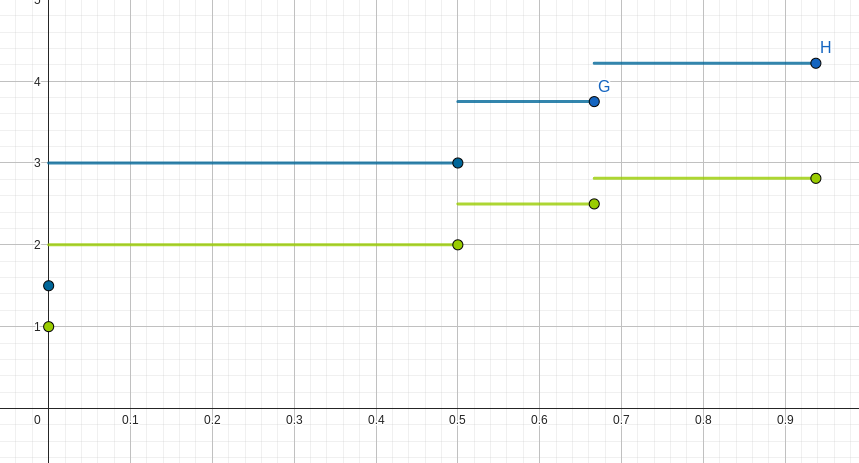
\includegraphics[width=1\linewidth]{fig2}
 	
 	
 	
 	
% \end{example} 




 \subsection{Operador de Poincaré} 
Llamaremos $\varphi_\alpha$ a solución  del problema de valores iniciales
 \begin{equation}
 	\left\lbrace \begin{array}{l}
 		d\varphi=f(t,\varphi(t))d\mu\\
 		\varphi(0)=\alpha,
 	\end{array}\right. \label{eq:Problema 0}
 \end{equation}
definida en \ref{def:sol}. De aquí  en adelante vamos a suponer que  $f:[0,T]\times\rr^n\to\rr^n$ está acotada, es decir $||f||_\infty<M$ y cumple con:
 \begin{enumerate}[label=\upshape(P-\arabic*),ref= (P-\arabic*)]
 	\item \label{pm1} Para cada $x\in\rr^n$, $f(t,x)$  $\mu$-medible en la variable $t$ y continua.
 	\item \label{pm2} Para cada $t\in[0,T]$, $f(t,x)$ es continua y acotada en la variable $x$.
 	\item \label{pm3} Existen $a,b$ positivos tal que
 	$$|f(t,x)|\leq a|x|+b.$$ 
 	\item \label{pm4}Existe $L\in\rr$ tal que $$\left| f(t,x)-f(t,y)\right|\leq L\left| x-y \right| . $$
 \end{enumerate} 
 Por el Teorema \ref{P-L}, para cada $\alpha$ existe una solución $\varphi_\alpha$ del problema de valores iniciales \eqref{eq:Problema 0}. Veamos qué propiedades tiene esta solución.
\begin{prop}
     Sea $\varphi_\alpha$ solución de  \eqref{eq:Problema 0}. Entonces $\varphi_{\alpha}\in L^\infty([0,T],\rr^n)$, y además si $s\leq t$, vale que
    \begin{equation*}\label{acotación}
        \left| \varphi_\alpha(t)-\varphi_\alpha(s)\right|\leq M\mu([s,t)).
    \end{equation*}
\end{prop}
\begin{proof}[Dem:]
 	Dado que $\varphi_{\alpha}$ es solución del problema \eqref{eq:Problema 0}, entonces por Definición  \ref{def:sol} tenemos que
 		$$\varphi_{\alpha}(t)=\varphi_{\alpha}(0)+\int_{[0,t)} f(s,\varphi_{\alpha}(s))\;d\mu,$$
 y por la desigualdad triangular vale que 
$$ 		|\varphi_{\alpha}(t)| \leq |\varphi_{\alpha}(0)|+\int_{[0,t)}| f(s,\varphi_{\alpha}(s))|\;d\mu.$$
Luego por \ref{pm3}
\begin{equation*}
\begin{split}
 	|\varphi_{\alpha}(t)| &\leq  |\varphi_{\alpha}(0)|+\int_{[0,t)}\left(a|\varphi_{\alpha}(s))|+b\right)\;d\mu\\	
     &\leq |\varphi_{\alpha}(0)|+b\mu([0,T])+a\int_{[0,t)}| \varphi_{\alpha}(s)|\;d\mu.
\end{split}
\end{equation*}
 Si llamamos $C=|\varphi_{\alpha}(0)|+b\mu([0,T])$ y $\nu=a\mu$, entonces
 $$|\varphi_{\alpha}(t)| \leq C+\int_{[0,t)}| \varphi_{\alpha}(s)|\;d\nu,$$
 aplicando el Teorema \ref{TG} obtenemos que para $t\in[0,T]$
 \begin{equation*}
 	|\varphi_{\alpha}(t)|\leq CK(T)\exp\left(K(T)a\bar{\mu}([0,T]) \right)  < \infty.
 \end{equation*}
Tomando supremo sobre todo el intervalo $[0,T]$, tenemos que\\
$\varphi_{\alpha}\in L^\infty([0,T],\rr^n).$
Por otro lado, como $||f||_\infty \leq M$, para $s\leq t$ vale que
  	\begin{equation*}
  		|\varphi_\alpha(t)-\varphi_\alpha(s)|\leq \int_{[s,t)}|f(r,\varphi_\alpha(r))|\;d\mu\leq M\;\mu\left( [s,t) \right). 
  	\end{equation*}
  
\end{proof}
\begin{cor}\label{corolario_continuidad}
    Sea $\varphi_\alpha$ solución de  \eqref{eq:Problema 0}. Si $t_0\in [0,T]$ cumple que $\mu(\{t_0\})=0$,  entonces $\varphi_\alpha$ es continua en $t_0$.
\end{cor}

\begin{proof}[Dem.]
Como $$0=\mu\left(\{t_0\}\right)=\mu\left(\bigcup_{n=1}^{\infty}\left[t_0-\frac{1}{n},t_0+\frac{1}{n}\right]\right)=\lim_{n\to\infty}\mu\left(\left[t_0-\frac{1}{n},t_0+\frac{1}{n}\right]\right)$$    
Para todo $\epsilon>0$ existe $N\in\nn$ tal que si $n>N$, entonces $$\mu\left(\left[t_0-\frac{1}{n},t_0+\frac{1}{n}\right]\right)<\epsilon/M.$$
Sea $\delta>0$ tal que  $\left[t_0-\delta,t_0+\delta\right]\subset\left[t_0-\frac{1}{n},t_0+\frac{1}{n}\right]$, entonces por la proposición \ref{acotación}, para $t\in \left[t_0-\delta,t_0+\delta\right]$ vale que
\begin{equation*}
    |\varphi_\alpha(t)-\varphi_\alpha(t_0)|\leq M\mu\left(\left[t_0-\frac{1}{n},t_0+\frac{1}{n}\right]\right)<\epsilon
\end{equation*}

\end{proof}




El siguiente teorema muestra que las soluciones de \eqref{eq:Problema 0}  están definidas en todo $[0,T]$.

 
 \begin{thm}[\textbf{Dominio de la solución}]\label{th:P(T)}
 	Sea $\mu$ una medida de Borel finita.   Si $f:[0,T]\times \rr^n\to\rr^n$  cumple con las condiciones \ref{pm1}  a \ref{pm4},  entonces la solución del problema \eqref{eq:Problema 0} está definida en todo el intervalo $[0,T]$.
 \end{thm}
 \begin{proof}[Dem.]
 	Supongamos que la solución máxima está definida en el intervalo $[0,t_1]$, donde $t_1< T$. Entonces por el Teorema  \ref{th:extensión} se debe cumplir alguna de las dos condiciones:
 	\begin{enumerate}
 		\item[A)] 	$\forall K\Subset [0,T)\times\rr^n$ existe $t_2\in [0,t_1)$ tal que $(t,\varphi(t))\notin K$   $\forall t\in(t_2,t_1)$. 

        \item[B)] Existe $x_1=\lim\limits_{t\to t_1^-}\varphi(t)$,  $(t_1,x_1)\in[0,T)\times\rr^n$ y  $$\left( t_1 , \varphi(t_1)+f(t_1,\varphi(t_1))\mu(\{t_1\})\right) \notin [0,T)\times\rr^n.$$
\end{enumerate}


   
 Si la condición (A) es verdadera, entonces para
 		$\epsilon\in\left( 0,\dfrac{T-t_1}{2}\right)$ 
    definimos el conjunto $K_{\epsilon}=[0,t_1+\epsilon]\times B(0,R)$ donde $||\varphi||_\infty\leq R$. Como $K_{\epsilon}$ es cerrado y acotado, entonces $K_{\epsilon}$ está compactamente incluido en $[0,T)\times\rr^n$. Luego existe $t_2\in [0,t_1)$ tal que $(t,\varphi(t))\notin K_{\epsilon}$ para todo $t\in(t_2,t_1)$.  Como $\varphi(t)\in B(0,R)$, la única manera de que  $(t,\varphi(t))\notin K_{\epsilon}$ es que  $t>t_1+\epsilon$, lo cual es un absurdo. Por otro lado, es inmediato que  (B) es falso,  porque si no lo fuese, resultaría que $\varphi(t_1)+f(t_1,\varphi(t_1))\mu(\{t_1\})\notin\rr^n$. Luego el intervalo donde está definida $\varphi$ es $[0,T]$.
 \end{proof}


\begin{defi} \label{def:op-poincare}
 Llamaremos operador de Poincaré  al operador $P:\rr^n\to \rr^n$ tal que para cada valor inicial $\alpha$,\index{operador de Poincaré} $P(\alpha)=\varphi_\alpha(T)$, \index[Simbolo]{$P$} donde $\varphi_\alpha$ es solución de \eqref{eq:Problema 0}.
\end{defi}

 
 \begin{lem}
    El operador de Poincaré es continuo.\label{opr continuo}
\end{lem}
\begin{proof}[Dem.]
 Sean $\varphi_\alpha$ y $\varphi_\beta$ dos soluciones del problema \eqref{eq:Problema 0}. Como $f$ es Lipschitz 
 \begin{equation*}
 \begin{split}
 	| \varphi_\alpha(t)-\varphi_\beta(t)|&\leq |\alpha-\beta |+\int_{[0,t)} |f(r,\varphi_\alpha(r)) -f(t,\varphi_\beta(t))| \; d|\mu|\\
	&\leq |\alpha-\beta|+L\int_{[0,t)} |\varphi_\alpha(r) -\varphi_\beta(t)| \; d|\mu|.
 \end{split}
\end{equation*}
 Si aplicamos el Teorema \ref{TG} tomando $u(t)=|\varphi_\alpha(t)-\varphi_\beta(t)|$, $c=|\alpha-\beta|$ y  $\nu=L|\mu|$, conseguimos

\begin{equation*}
|\varphi_\alpha(t)-\varphi_\beta(t)|\leq K(t) |\alpha-\beta|e^{K(t)L\bar{|\mu|}([t_0,t))}.
\end{equation*}
Luego, si evaluamos en $t=T$ y llamamos  $K=K(T)=\displaystyle\prod_{\tau\in D}\mu(\{\tau\})<\infty$.
 

\begin{equation*}
 		|P(\alpha)-P(\beta)|=|\varphi_{\alpha}(T)-\varphi_{\beta}(T)|_{1}\leq K |\alpha-\beta|_{1}e^{KL\bar{|\mu|}([0,T))}\to 0
 	\end{equation*}
 cuando $|\alpha-\beta|\to 0$.
\end{proof}
 
 
 

%\begin{obs} \label{ob: cont P}
 %	Por \ref{th:P(T)}  el operador de Poincaré está bien definido, ya que la solución se puede extender a todo el intervalo $[0,T]$. Además por \ref{opr continuo} el operador es continuo.
 %\end{obs} 
 
 

 \begin{thm} \label{th: P}
 	Sea $R>0$ y $f$ satisface las condiciones \ref{pm1} a \ref{pm4}, \ref{fun-tele} para $B(0,R)$  y  además que
 	\begin{equation}
 		f(t,u)\cdot u<0 \text{ para todo par } (t,u) \text{ donde }  |u| =R  \text{ y   } \mu(\{t\})=0.  \label{eq:4}
 	\end{equation}
 Entonces el operador de Poincaré definido en \ref{def:op-poincare} cumple que \\
 $P\left(  \overline{B(0,R)}\right)  \subset \overline{B(0,R)}$.
 \end{thm}
 
 \begin{proof}[Dem.] Sea $\varphi_\alpha$  la solución a \ref{eq:Problema 0} y sea $A=\{t\in [0,T] \mid \varphi_\alpha(s)\in \overline{B(0,R)}, \; \forall s\in [0,t]\}$, veamos que el conjunto $A$ es simultáneamente abierto y cerrado relativo al intervalo $[0,T]$, y  como $[0,T]$ es conexo, entonces $A=[0,T]$.
  
 Veamos primero que  $A$  es un conjunto cerrado respecto al $[0,T]$. Para ello, sea   $t_n$  una sucesión de $A$ que converge a $t$, veamos que $t\in A$.  Si para algún $n$, $t_n\geq t$ entonces $\forall s \in [0,t]\subset [0,t_n] $ vale que $\varphi_\alpha(s)\in\overline{B(0,R)}$,  por lo tanto en $t\in A$.  Si por el contrario $\forall n$ tenemos que $t_n < t$,  como $\varphi_\alpha$ es continua a izquierda, entonces $\lim\limits_{n\to \infty}\varphi_\alpha(t_n)=\varphi_\alpha(t)$ y como cada $\varphi_\alpha(t_n)\in \overline{B(0,R)}$ es inmediato que $\varphi_\alpha(t)\in \overline{B(0,R)}$, es decir $t\in A$.  Por lo tanto, $A$ es cerrado.
 	 
  	Si $A$ es un conjunto abierto relativo al $[0,T]$, entonces $[0,T]\setminus A$ es cerrado, es decir para toda sucesión $\{t_n\}\subset [0,T]\setminus A$ si $t_n\to t$ entonces $t\in[0,T]\setminus A$. Por lo tanto si suponemos que  $A$ no es abierto relativo al intervalo $[0,T]$, entonces $\exists t_0\in A$ y $\{t_n\}\nsubset A$ tal que $t_n\to t_0$. Podemos asegurar que si $t> t_0$ entonces $t\notin A$, pues existe $n_0$ tal que $t_0<t_{n_0}<t$ y como tengo que $t_{n_0}\notin A$, en particular $|\varphi_\alpha(t_{n_0})|>R$.
   
   Veamos que como $t_0\in A$, entonces $\varphi_\alpha(t_0)\in B(0,R)$ o  $\varphi_\alpha(t_0)\in \partial B(0,R) $, y siempre existe $t> t_0$ tal que $t\in A$.%$|\varphi(t)|\in \overline{B(0,R)}$.% 
 		\begin{itemize}
   		\item Supongamos que $\varphi_\alpha(t_0)\in B(0,R)$.
     \end{itemize}
En el problema \eqref{eq:Problema 0} podemos tomar como condición inicial $\varphi(0)=\varphi_\alpha(t_0)=\beta\in B(0,R)$, entonces por el Teorema \ref{P-L} existe una solución, que notaremos  $\varphi_{\beta}$. Luego, tenemos que para todo $t\in [0,\delta)$ el par $(t,\varphi_\beta(t))\in \Omega$, donde  $\Omega$ es un entorno de $[0,T]\times B(0,R)$. Ahora podemos extender a $\varphi_\alpha $ de la siguiente manera
$$\varphi_\alpha(t)=\left\{\begin{array}{ccc}
    \varphi_\alpha(t) & si &  t\in[0,t_0)\\
     \varphi_\beta(t-t_0) & si &t\in[t_0,t_0+\delta) 
\end{array}\right.$$
Por lo tanto para todo $t\in[t_0,t_0+\delta)$ vale que $|\varphi_\alpha(t)|=|\varphi_\beta(t-t_0)|\leq R$. Es decir existe $t>t_0$ tal que $t\in A$.

    
    \begin{itemize}
        
    
    \item Supongamos que  $\varphi(t_0)\in \partial B(0,R)$ y $\mu(\{t_0\})\neq 0$.
    
    \end{itemize}
Por \eqref{fun-tele}  $x_1=\varphi(t_0)+f(t,\varphi(t_0))\mu(\{t_0\})\in B(0,R)$, y tomando la medida $\hat{\mu}=\mu-\mu(\{t_0\})\delta_{t_0}$, es claro que $\hat{\mu}(\{t_0\})=0$, puedo aplicar el Teorema \ref{P-L} para la condición inicial $\varphi(0)=x_1$, pero con la medida $\hat{\mu}$.  Luego, existe $\delta>0$  y $\varphi_{x_1}$ tal que $|\varphi_{x_1}(t)|\leq R$ para todo $t\in [0,0+\delta)$. Ahora puedo extender la solución $\varphi_\alpha$ al intervalo $[0,t_0+\delta)$  de la siguiente manera
$$\varphi_\alpha(t)=\left\{\begin{array}{ccc}
    \varphi_\alpha(t) & si &  t\in[0,t_0]\\
     \varphi_{x_1}(t-t_0) & si &t\in(t_0,t_0+\delta) 
\end{array}\right.$$
Por lo tanto existe $t>t_0$ tal que $|\varphi_\alpha(t)|<R$, es decir vale que $t\in A$.



% \begin{multline*}
 %	|\hat{\mu}|\left( \{t_0\}\right) =|\hat{\mu}|\left( \bigcap_{n=1}^\infty[t_0,t_0+1/n)\right)=\lim\limits_{n\to\infty}|\hat{\mu}|\left( [t_0,t_0+1/n) \right) =0
 %\end{multline*} 
 %existe $N>0$ que $|\hat{\mu}\left( [t_0,t_0+1/N]\right)\leq R/M $. Por lo tanto puedo aplicar el Teorema de Existencia y Unicidad para las condiciones $(t_0,x_1)$ y la medida $\hat{\mu}$, por el cual va a  existir $\delta$ tal que el problema \refeq{Problema P} tiene solución en el intervalo $[t_0,t_0+\delta]$,  es decir podemos extender la solución del problema hasta el intervalo $[0,t_0+\delta]$ lo cual contradice que $A$ no sea abierto.
 		



    
\begin{itemize}
\item Supongamos $\varphi(t_0)\in \partial B(0,R)$ y $\mu(\{t_0\})= 0$ 
\end{itemize}
De \eqref{eq:4} existe $b>0$ tal que $f(t_0,\varphi(t_0))\cdot\varphi(t_0)<-b$.

Por \eqref{f lipschitz} y Corolario \ref{corolario_continuidad}, para $\epsilon=\frac{b}{3RL}$ existe $\delta_1>0$ tal que si $t\in[t_0,t_0+\delta_1)$ entonces
\begin{equation}
    \begin{split}
        \int_{[t_0,t)} f(s,\varphi_\alpha(s))-f(s,\varphi_\alpha(t_0))\; d\mu& \leq \int_{[t_0,t)} |\varphi_\alpha(s)\varphi_\alpha(t_0)|\; d\mu \\ &\leq \frac{b}{3R}\mu((t_0,t)).
    \end{split}\label{eq:A}
\end{equation}
Además, como $f$ es continua en $t_0$ $\exists \delta_2>0 $ tal que si $s\in [t_0,t_0+\delta_2)$, entonces
\begin{equation}
    |f(s,\varphi_\alpha(t_0))-f(t_0,\varphi_\alpha(t_0))|\leq \frac{b}{3R}.\label{eq:B}
\end{equation}

Para todo $t\in[t_0,t_0+\delta)$, donde $\delta=\min\{\delta_1,\delta_2\}$, usando \eqref{eq:A} y \eqref{eq:B} tenemos que 
\begin{equation*}
    \begin{split}
    \varphi_\alpha(t)-\varphi_\alpha(t_0) &= \int_{(t_0,t)}\left[f(s,\varphi_\alpha(s))-f(s,\varphi_\alpha(t_0))\right]\; d\mu\\& + \int_{(t_0,t)}\left[f(s,\varphi_\alpha(t_0))-f(t_0,\varphi_\alpha(t_0))\right]\; d\mu \\&+ \int_{(t_0,t)}f(t_0,\varphi_\alpha(t_0))\; d\mu,\\
& \leq \frac{b}{3R}\mu((t_0,t)) + \int_{(t_0,t)}\frac{b}{3R}\; d\mu + \int_{(t_0,t)}f(t_0,\varphi_\alpha(t_0))\; d\mu.
\end{split}
\end{equation*}		 
Si multiplicamos por el vector $\varphi_\alpha(t_0)$ y como $|\varphi_\alpha(t_0)|=R$, entonces
\begin{equation*}
\begin{split}
\left[\varphi_\alpha(t)-\varphi_\alpha(t_0)\right]\cdot \varphi_\alpha(t_0) \leq & \varphi_\alpha(t_0)\frac{2b}{3R}\mu((t_0,t))\\& + \int_{(t_0,t)}f(t_0,\varphi_\alpha(t_0))\cdot \varphi_\alpha(t_0)\; d\mu\\
&\leq \frac{2b}{3}\mu((t_0,t))-b\mu((t_0,t))=-\frac{b}{3}\mu((t_0,t)).
\end{split}
\end{equation*}
Luego por la Proposición?? \eqref{acotación}
\begin{equation*}
    \begin{split}
    |\varphi_\alpha(t)|^2=&|\varphi_\alpha(t_0)|^2+2\left[\varphi_\alpha(t)-\varphi_\alpha(t_0)\right]\cdot\varphi_\alpha(t_0)+|\varphi_\alpha(t)-\varphi_\alpha(t_0)|^2\\
   &\leq R^2-\dfrac{2b}{3}\mu((t_0,t))+M^2 \mu((t_0,t))^2.  
    \end{split}
\end{equation*}
O equivalentemente
\begin{equation}
    |\varphi_\alpha(t)|^2-R^2\leq \mu((t_0,t))\left[M^2 \mu((t_0,t))-\dfrac{2b}{3}\right]. 
\end{equation}
El término de la derecha es una expresión cuadrática respecto a $\mu((t_0,t))$, y tiene como raíces $t_0$ y  otro valor a derecha de $t_0$, es decir existe $t_1>t_0$ tal que $|\varphi_\alpha(t_1)|^2-R^2\leq 0$, por lo tanto $t_1\in A$.
  		
Por lo tanto, mostramos que existe $t_1>t_0$ tal que $t\in A$, lo cual contradice que no sea abierto relativo al $[0,T]$. Finalmente, si $A$ es abierto y cerrado relativo al intervalo $[0,T]$, entonces $A=[0,T]$.
 	
Luego, para cualquier $\alpha\in\overline{B(0,R)}$, $$P(\alpha)=\varphi_\alpha(T)\in\overline{B(0,R)}.$$ 
 \end{proof}
 
 \begin{thm}[\textbf{Teorema de Brouwer}]
 	
 	Sea $B(0,R)$ una bola de $\rr^n$  y sea $P:\overline{B(0,R)}\to \overline{B(0,R)}$ continua. Entonces existe $x \in \overline{B(0,R)}$ tal que $P(x) = x$.
 \end{thm}
 \begin{thm} \label{th:final}
 	Sea $\mu$ una medida de Borel finita, y sea $f:[0,T]\times\rr^n\to\rr^n$ una función que cumple con las condiciones \ref{pm1} a \ref{pm4}. Además, existe una bola $B(0,R)$ tal que si $x\in\overline{B(0,R)}$, entonces
    $x+f(t,x)\mu(\{t\})\in \overline{B(0,R)}$ para todo $t\in[0,T]$, y
 	$$f(t,x)\cdot x<0 \; \text{ para todos}\; |x|=R \;\text{y}\; \mu(\{t\})=0.$$
 	Entonces el problema
 	 \begin{equation}
 		\left\lbrace \begin{array}{l}
 			d(\varphi)=f(t,\varphi(t))d\mu\\
 			\varphi(0)=\varphi(T)
 		\end{array}\right. \tag{${PP}$}
 	\end{equation} 
tiene al menos una solución. 
\end{thm}
 \begin{proof}[Dem.]
 	Por el Teorema \ref{th:P(T)} y el Lema  \ref{opr continuo}, el operador $P$ está bien definido y es continuo. Luego, por el Teorema  \ref{th: P} se tiene que $P\left( \overline{B(0,R)}\right)\subset\overline{B(0,R)} $, y ahora aplicando el Teorema de Brouwer  se llega a que existe una solución $\varphi$ al problema \eqref{eq:Problema 0} tal que $\varphi(T)=\varphi(0).$
 \end{proof}

 \begin{example}\label{ejemplo vectorial}
 	Sea $u:[0,T]\to \rr$, y sean $g_{1,2}:[0,T]\to \rr^n$  funciones suficientemente buenas, definimos el siguiente problema impulsivo
 	 \begin{equation}\label{eq:ejemplo 3}
 		\left\lbrace \begin{array}{l}
    u''=g_1(t,u,u')d\lambda+g_2(t,u,u') \displaystyle\sum_{i=1}^rd\delta_{t_i}\\
 			u'(0)=u'(T)\\
 			u(0)=u(T),
 		\end{array}\right. 
 	\end{equation} 
 donde $t_i\in(0,T)$ y $\delta_{t_i}$ es la medida delta de Dirac concentrada en $t_i$. Veamos como podemos aplicar el teorema \ref{th:final} a este tipo de problemas.
 
 Si llamamos $u'=v$  podemos transformar el problema \eqref{eq:ejemplo 3} en un sistema de ecuaciones
  \begin{equation*}
 	\left\lbrace \begin{array}{l}
 		(u',v')=\left(v, g_1(t,u,v)\right)d\lambda +\displaystyle\sum_{i=1}^r\left(0,g_2(t,u,v)\right)d \delta_{t_i}\\
   (u(0),v(0))=(u(T),v(T)).
 	\end{array}\right. 
 \end{equation*} 
A este sistema de ecuaciones lo podemos escribir de manera vectorial, tomando $\varphi=(u,v)$, $G_1(t,\varphi)=(v,g(t,u,v))$ y $G_2(t,\varphi)=(0,g_2(t,u,v))$.
  \begin{equation*}
	\left\lbrace \begin{array}{l}
	\varphi'=G_1(t,\varphi)d\lambda+G_2(t,\varphi)\displaystyle\sum_{i=1}^r d \delta_{t_i}\\
 \varphi(0)=\varphi(T).
	\end{array}\right. 
\end{equation*} 
Si llamamos $F(t,\varphi)=\left( G_1(t,\varphi)\chi_{[0,T]-\{t_1,..,t_r\}}+G_2(t,\varphi)\chi_{\{t_1,...,t_r\}}\right) $ y tomando $d\mu=d\left(\lambda+\displaystyle\sum_{i=1}^r\delta_{t_i}\right)$, entonces la ecuación vectorial se transforma en la del Teorema \ref{th:final}. 
 \end{example}

 \chapter{Experimentos Numéricos}

En este capítulo vamos a desarrollar un método numérico para hallar soluciones a MDE mediante el método shooting. Primero haremos una descripción del método y luego analizaremos la convergencia del mismo. En apéndice  \ref{apendice A} mostraremos el código que utilizamos, escrito en lenguaje Pyhton.

\section{Método Numérico }



Como ya dijimos, el método shooting consiste en resolver la MDE
\begin{equation}\label{eq:P}
\left\lbrace \begin{array}{lc}
d\varphi=f(t,\varphi) d\mu& \text{ para } t\in [0,T]\\
\varphi(0)=\alpha,
\end{array}\right. \tag{$P$}
\end{equation} 
para varios valores de $\alpha$ y ver para cuál se cumple que  $\alpha=\varphi(T)$.

De acuerdo a  la Definición \ref{def:sol},  una solución de \eqref{eq:P} es una función $\varphi\in  BV([0,T],\rr^n)$ y continua izquierda tal que
\begin{equation}\label{eq:integral}
    \varphi(t)=\alpha+\int_{[0,t)}f(s,\varphi(s)) \;d\mu.
\end{equation}
El procedimiento consta de dos partes. En la primera se aproxima la solución al problema de valores iniciales \ref{eq:P} mediante iteraciones sucesivas de Picard \cite{Simmons}, las cuales se generan de la siguiente manera
\begin{equation*}
    \begin{split}
        &\varphi_0=\alpha\\
        &\varphi_k(t)=\alpha+\int_{0,t}f(s,\varphi_{k-1}(s)) \,d\mu.
    \end{split}
\end{equation*}
\textcolor{blue}{En \cite{P.Mazzone} los autores muestran que   las iteraciones de Picard convergen  a la solución en un caso más general, en el Teorema \ref{th:picar} mostraremos la convergencia en nuestro caso particular y además veremos con qué velocidad converge}. 

La segunda parte consiste en aproximar el término de la derecha de \eqref{eq:integral}, el cual es una integral en el sentido de Labesgue-Stieljes. Para aproximar la integral de (L-S) usaremos  sumas de Riemann-Stieljes, de la siguiente manera
\begin{equation}\label{eq:4.1.2}
    \int_{[0,t)}f(s,\varphi(s))\; d\mu \approx \sum_{k=1}^{n-1}f(t_k,\varphi(t_k))\mu\left([t_k,t_{k+1})\right),
\end{equation}
donde los puntos $\{t_k\}$ son una partición del intervalo $[0,t]$. Cabe aclarar que la función  que estamos integrando no es necesariamente  integrable en el sentido de la integral de Riemann-Stieljes (R-S)\index[Simbolo]{(R-S)}. Para que la integral de (R-S) exista es suficiente que la función sea continua \cite{Lakshmikan} o el conjunto de discontinuidades tenga medida cero con respecto a la medida $\mu$ \cite{Hobson}, lo cual por lo general no pasa. En el Teorema \ref{th:R-S} veremos que cuando evaluamos la función en el miembro de la izquierda  de \eqref{eq:4.1.2}, la suma de (R-S) efectivamente converge a la integral de (L-S).





%\section{Convergencia del método}
\begin{thm}\label{th:R-S}
    Sea $F:[0,T]\times \rr^n\to \rr^n$ continua  izquierda y sea $\mu$ una medida de Borel positiva y finita. Supongamos que existe $M>0$ tal que $|F|<M$. Entonces para todo $\epsilon>0$ y para cualquier partición del intervalo $[0,T]$, $P_n=\{0=t_1, t_2, \ldots, t_n=T\}$, existe $\delta>0$ tal que 
      \begin{equation*}
    \left|\int_{[0,T)}F(s)\; d\mu - \sum_{k=1}^{n-1}F(t_k)\mu\left([t_k,t_{k+1})\right)\right|<\epsilon,
\end{equation*}   
siempre que $\max\{t_{k+1}-t_k\}<\delta$.
\textcolor{blue}{Así está bien?}
\end{thm}
\begin{proof}[Dem.]
Supongamos que la afirmación es falsa, entonces para todo $\in\nn$ existe una partición $P^n_k=\{0=t^n_1, t^n_2, \ldots, t^n_k=T\}$ del intervalo $[0,T]$ tal que $\max\{t_{k+1}-t_k\}<1/n$ y
\begin{equation}\label{eq:4.6}
    \left|\int_{[0,T)}F(s)\; d\mu - \sum_{k=1}^{n-1}F(t_k)\mu\left([t_k,t_{k+1})\right)\right|>\epsilon.
\end{equation}    
Si armamos la función simple 
$$\Phi(t)=\sum_{k=1}^{n-1}F(t_k) \chi_{[t^n_k,t^n_{k+1})}$$
para cada $t\in[0,T]$ existe un intervalo de la partición $P^n_k$ tal que $t\in[t_k,t_{k+1})$ y además $t-1/n<t^n_k$, por lo tanto $t^n_k$ tiende a $t$ por izquierda cuando $n\to \infty$. Como $F$ es continua a izquierda, tenemos que
\begin{equation*}
\begin{split}
    |\Phi(t)-F(t)|=\left|\sum_{k=1}^{n-1}[F(t_k)-F(t)] \chi_{[t^n_k,t^n_{k+1})} \right|\leq |F(t^n_k)-F(t)|\to 0
\end{split}
\end{equation*}
Luego, como $|F|<M$ entonces $|\Phi|<M$ y por el Teorema de la convergencia mayorada de Lebesgue 
\begin{equation*}
\begin{split}
    \int_{[0,T)}F(t)\, d\mu&=\lim_{n\to \infty}\int_{[0,T)}\Phi(t)\, d\mu=\lim_{n\to \infty}\int_{[0,T)}\sum_{k=1}^{n-1}F(t_k) \chi_{[t^n_k,t^n_{k+1})}\, d\mu \\ &=\lim_{n\to \infty}\sum_{k=1}^{n-1}F(t_k) \mu([t^n_k,t^n_{k+1})).
\end{split}
\end{equation*}
Llegamos a un absurdo, pues se contradice \eqref{eq:4.6}
\end{proof}
Antes de ver el caso particular de las iteraciones de Picard, vamos a enunciar el Teorema de punto fijo de Banach cuya demostración se puede ver en \cite{Amster}.
\begin{thm}[Punto Fijo de Banach]
Sea $\mathcal{X}$ un espacio métrico completo, $T:\mathcal{X}\to \mathcal{X}$ y  $\exists K<1$ tal que 
\begin{equation*}
    d(T[x],T[y])\leq Kd(x,y)    
\end{equation*}
para todo $x,y\in \mathcal{X}$. Entonces $T$ tiene un único punto fijo $\tilde{x}$. Además, si $x_0\in \mathcal{X}$ es un punto arbitrario y $\{x_{n}\}_n^\infty=0$, la sucesión recursiva definida como   $x_n=T(x_{n-1})$, entonces $\tilde{x}=\lim_{n\to \infty}x_n$.
\end{thm}
El siguiente corolario es muy útil para definir las iteraciones de Picard.
\begin{cor}\label{col:picard}
Sea $\mathcal{X}$ un espacio métrico completo. Definimos  $T^n=T\circ T\circ ...\circ T$ ($n$-veces) y además $\exists K<1$ tal que 
    \begin{equation*}
    d(T^n[x],T^n[y])\leq Kd(x,y)    
    \end{equation*}
para todo $x,y\in \mathcal{X}$ y para todo $n$. Entonces $T$ tiene un único punto fijo en $\mathcal{X}$.
\end{cor}
 

\newpage
\begin{thm}\label{th:picar}
    Sea $\mu$ una medida de Borel finita y positiva en $[0,T]$, y sea $f:[0,T]\times\rr^n\to\rr^n$ continua y que satisface \ref{f lipschitz},\comment{Cuando cites ecuaciones usa el comando \texttt{$\backslash$ eqref}, asi el lector sabe que tiene que buscar una ecuación y no un enunciado. Otra cosa, me parece que faltan hipótesis para $f$. En vistas de este teorema que citas, tenemos que analizar si incluir el que enunciasnte en un capítulo anterior } entonces el problema \eqref{eq:P} tiene una única solución, es decir existe una única función $\varphi\in BV([0,T],\rr^n)$, continua a izquierda tal que 
 
    \begin{equation*}
        \varphi(t)=\alpha + \int_{[0,t)}f(s,\varphi(s))\, d\mu.
    \end{equation*}
\end{thm}
\begin{proof}[Dem.] %\vphantom{a}\\
Sea $$\mathcal{X}=BV_\alpha([0,T],\rr^n)\cap \{\varphi:[0,T]\to \rr^n \mid \varphi \text{ es continua a izquierda}\}.$$
Definimos el operador $T$, como 
\begin{equation}\label{eq:T}
    T[\varphi]= \alpha + \int_{[0,t)}f(s,\varphi(s))\, d\mu.
\end{equation}
Entonces, un punto fijo de $T$ será la solución que estamos buscando. Veamos las siguientes afirmaciones.

\begin{enumerate}
    \item
    \textbf{$\mathcal{X}$ es completo con la métrica $d$.} 
    
    En la proposición \ref{pro:completo}, vimos que $(BV_\alpha([0,T],\rr^n),d)$ es completo. Veamos que $\mathcal{X}$ es un subconjunto cerrado de $BV_\alpha([0,T],\rr^n)$ y por lo tanto completo. Sea $\{\varphi_n\}\subset \mathcal{X}$ ta que $d(\varphi_n, \varphi_0) \to 0$, entonces $\varphi_0\in BV_\alpha([0,T],\rr^n)$. Además, para cualquier $\epsilon>0$  existe $n_0$, tal que $\forall n>n_0$ vale que $d(\varphi_0,\varphi_n)<\epsilon/2$. Luego, para cualquier $t\in[0,T]$, tenemos que
    \begin{equation*}
        \begin{split}
            |\varphi_0(t-1/n)-\varphi_0(t)|&\leq 
            |\varphi_0(t-1/n)-\varphi_n(t-1/n)|\\&+|\varphi_n(t-1/n)-\varphi_n(t)|+|\varphi_n(t)-\varphi_0(t)|\\
            &\leq d(\varphi_0,\varphi_n)+|\varphi_n(t-1/n)-\varphi_n(t)|+d(\varphi_n,\varphi_0)\\
            &\leq \epsilon +|\varphi_n(t-1/n)-\varphi_n(t)|.
        \end{split}
    \end{equation*}
Como $\varphi_n$ es continua a izquierda, podemos concluir que $\varphi_0\in \mathcal{X}$. Luego $\mathcal{X}$ es un subconjunto cerrado de un espacio completo, por lo tanto también es completo.

\item  \textbf{El operador $T$ está bien definido.}

Si $\varphi \in \mathcal{X}$, entonces para cualquier $t\in[0,T]$ vale que
\begin{equation}\label{afi2.1}
    |\varphi(t)|\leq |\varphi(0)|+ V(\varphi,[0,T]),
\end{equation}
es decir $\varphi$ está acotada. Por otro lado, como $f$ es Lipschitz
\begin{equation}\label{afi2.2}
\begin{split}
    |f(t,x)|&\leq |f(t,x)-f(t,0)|+ |f(t,0)|\\
    &\leq L|x|+|f(t,0)|,
\end{split}
\end{equation}
y además, dado que $f$ es continua existe $a>0$ tal que $|f(t,0)|<a$ para todo $t\in [0,T]$. Entonces por \eqref{afi2.1} y \eqref{afi2.2} para todo $t\in[0,T]$ verifica que
\begin{equation*}
    |f(t,\varphi(t)|\leq L|\varphi(t)|+|f(t,0)|\leq L\left(|\varphi(0)+V(\varphi,[0,T]) \right) +a.
\end{equation*}
Si llamamos \index[Simbolo]{$A_\varphi$} $A_\varphi=L\left(|\varphi(0)+V(\varphi,[0,T]) \right) +a$, entonces
\begin{equation}\label{afi3.1}
\begin{split}
    \int_{[0,t)}f(s,\varphi(s))\, d\mu\leq A_\varphi\mu([0,t))<\infty,
\end{split}
\end{equation}
es decir,  $T[\varphi]<\infty$ para toda $\varphi\in \mathcal{X}$. 

\item \textbf{Sea $\varphi\in \mathcal{X}$, entonces $T[\varphi]\in \mathcal{X}$. } 

Primero observemos que $T[\varphi]\in BV_\alpha([0,T],\rr^n)$. Sea $P_n=\{t_k\}_{k=1}^n$ una partición del intervalo $[0,T]$, entonces usando \eqref{afi3.1} y que $\mu$ es positiva, 
\begin{equation*}
    \begin{split}
        \sum_{k=1}^{n-1}|T[\varphi](t_{k+1})-T[\varphi](t_{k})|&\leq \sum_{k=1}^{n-1}\int_{[t_k,t_{k+1})}|f(s\varphi(s)|\, d\mu, \\
        &\leq A_\varphi\mu([0,T))<\infty.
    \end{split}
\end{equation*}


Como el miembro de la derecha no depende de la partición, cuando tomamos supremo sobre todas las particiones del intervalo $[0,T]$, tenemos que
\begin{equation*}
    V(T[\varphi],[0,T])<\infty.
\end{equation*}
Además $T[\varphi](0)=\alpha$, por lo tanto $T[\varphi]\in BV_\alpha([0,T],\rr^n)$.

Por último,  mostremos que $T[\varphi]$ es continua a izquierda. Sea $t_n \to t^-$, entonces como $[t_{n+1},t)\subset [t_n,t)$ por \cite[3.28]{Zo}

\textcolor{red}{qué es (3.28) en la referencia? Ecuación, Teorema, Lema?}\textcolor{blue}{no dice..}
\begin{equation*}
    \lim_{n\to \infty}\mu([t_n,t))=\mu\left(\bigcap_{n=1}^\infty[t_n,t)\right)=\mu(\emptyset)=0.
\end{equation*}
Luego por \eqref{afi3.1}
\begin{equation*}
\begin{split}
    \left|\int_{[0,t_n)}f(s,\varphi(s))\, d\mu - \int_{[0,t)}f(s,\varphi(s))\, d\mu   \right|&\leq \int_{[t_n,t)}|f(s,\varphi(s))|\, d\mu \\ &\leq A_\varphi\mu([t_n,t))\to 0,
\end{split}
\end{equation*}
es decir $T[\varphi](t_n)\to T[\varphi](t)$.

\item \textbf{Sea $T^n=T\circ T\circ ...\circ T$ ($n$-veces). Mostremos que  para cualquier $\varphi_1,\varphi_2\in \mathcal{X}$, $\exists L>0$ tal que }
\begin{equation}\label{eq:4.3.1}
d(T^n[\varphi_1],T^n[\varphi_2]\leq \dfrac{L^{n}\left[\mu([0,T))\right]^{n}}{n!} d(\varphi_1,\varphi_2),
\end{equation}


Para $n=0$ es claro que \eqref{eq:4.3.1} se verifica pues
\begin{equation*}
    \begin{split}
d(T^0[\varphi_1],T^0[\varphi_2])&=V(T^0[\varphi_1]-T^0[\varphi_2],[0,T])=V(\varphi_1-\varphi_2,[0,T])\\ & =d(\varphi_1,\varphi_2).
\end{split}
\end{equation*}
Supongamos válida la desigualdad \eqref{eq:4.3.1} para $n$ y probemos que vale para $n+1$.
Sea $\{t_i\}_{i=1}^k$ una partición del intervalo $[0,T]$. Como $f$ es Lipschitz, entonces existe $L>0$ tal que
\begin{equation*}
    \begin{split}
        &\sum_{i=1}^{k-1}\left|T^{n+1}[\varphi_1](t_{i+1})-T^{n+1}[\varphi_2](t_{i+1})-T^{n+1}[\varphi_1](t_{i})+T^{n+1}[\varphi_2](t_{i})  \right|\\
        &\leq \sum_{i=1}^{k-1}\int_{[t_i,t_{i+1})}\left| f(s,T^n[\varphi_1](s))-f(s,T^n[\varphi_2](s))  \right|\, d\mu\\
        &\leq \sum_{i=1}^{k-1}L\int_{[t_i,t_{i+1})}\left| T^n[\varphi_1](s)-T^n[\varphi_2](s)  \right|\, d\mu \\ 
        &\leq L\int_{[0,T]}\left| T^n[\varphi_1](s)-T^n[\varphi_2](s)  \right|\, d\mu.
    \end{split}
\end{equation*}
Además, por el lema \ref{lem:var-acotada} se verifica que 
$$|T^n[\varphi_1](s)-T^n[\varphi_2](s)|\leq d(T^n[\varphi_1],T^n[\varphi_2]),$$
y como supusimos que la desigualdad \eqref{eq:4.3.1} 
vale para $n$, entonces
\begin{equation*}
    \begin{split}
        &\sum_{i=1}^{k-1}\left|T^{n+1}[\varphi_1](t_{i+1})-T^{n+1}[\varphi_2](t_{i+1})-T^{n+1}[\varphi_1](t_{i})+T^{n+1}[\varphi_2](t_{i})  \right|\\
        &\leq L\int_{[0,T]}\left| T^n[\varphi_1](s)-T^n[\varphi_2](s)  \right|\, d\mu \leq L\int_{[0,T]}d(T^n[\varphi_1],T^n[\varphi_2])\, d\mu \\ &\leq \dfrac{L^{n+1}d(\varphi_1,\varphi_2)}{n!}\int_{[0,T]}\left[\mu([0,s))\right]^n\, d\mu.
    \end{split}
\end{equation*}
Luego, si tomamos supremo sobre todas las particiones del intervalo $[0,T]$ obtenemos que
\begin{equation*}
    \begin{split}
d(T^{n+1}[\varphi_1],T^{n+1}[\varphi_2]) &\leq \dfrac{L^{n+1}d(\varphi_1,\varphi_2)}{n!}\int_{[0,T]}\left[\mu([0,s))\right]^n\, d\mu.
    \end{split}
\end{equation*}
Aplicando la observación \ref{Teorema 6.1}, tomando $F=\dfrac{x^{n+1}}{n+1}$ y $g(s)=\mu([0,s))$, tenemos que
\begin{equation*}
    \begin{split}
d(T^{n+1}[\varphi_1],T^{n+1}[\varphi_2]) &\leq \dfrac{L^{n+1}d(\varphi_1,\varphi_2)}{n!}\dfrac{\left[\mu([0,T])\right]^{n+1}}{n+1}\\
&\leq \dfrac{L^{n+1}\left[\mu([0,T])\right]^{n+1}}{(n+1)!}d(\varphi_1,\varphi_2).
    \end{split}
\end{equation*}

\end{enumerate}
Luego $T$ cumple con las hipótesis del corolario \ref{col:picard} y existe $\varphi\in\mathcal{X}$ tal que $T[\varphi]=\varphi$. Es decir, existe $\varphi\in BV([0,T],\rr^n)$, continua a izquierda tal que $\varphi(0)=\alpha$ y para todo $t\in[0,T]$ vale que
$$\varphi(t)=\alpha\int_{[0,t)}f(s,\varphi(s) \, d\mu.$$
\end{proof}

\begin{cor}[Velocidad de convergencia]
Si estamos en las condiciones del Teorema \ref{th:picar} y $\varphi$ es un punto fijo de $T$, definido como \eqref{eq:T}. Entonces para cualquier $\varphi_1\in BV_\alpha([0,T],\rr^n)$ y continua a izquierda, \textcolor{red}{vale} que
    \begin{equation}
    |T^n[\varphi_1](t)-\varphi(t)|\leq \dfrac{\left(L\mu([0,T])\right)^n}{n!}d(\varphi_1,\varphi)   ,     
    \end{equation}
para todo $t\in[0,T].$
\end{cor}
\begin{proof}[Dem.]
La desigualdad se deduce del Teorema \ref{th:picar} y del Lema \ref{lem:var-acotada}.
\end{proof}






\section{Simulaciones}

Aplicamos el método shooting para problemas como los descriptos en el ejemplo \ref{ejemplo vectorial}. En particular\textcolor{red}{,} \underline{queríamos}

\textcolor{red}{en pasado?...aunque se haya hablado del tema en la intro, si presenta a continuación el sistema...convendría escribir en presente o futuro: queremos/querremos} 

hallar soluciones periódicas para la ecuación de un péndulo forzado sin rozamiento, donde la fuerza externa que actúa es una fuerza impulsiva.

\textcolor{red}{Algo para presentar lo que sigue???  : (dos puntos) en lugar del . (punto seguido), ó cambiar el punto seguido por  '' , como/ del estilo de''  }
\begin{equation}\label{eq:pendulo}
	\left\lbrace \begin{array}{l}
	u''(t)=-sen(u(t))+\displaystyle\sum_{i=1}^r d \delta_{t_i} \mbox{ con } t\in[0,4\pi]\\
 u'(0)=u'(4\pi)\\
 u(0)=u(4\pi).
	\end{array}\right.
\end{equation} 
Si $u'=v$ y llamando $\varphi=(u,v)$, entonces una solución de \eqref{eq:pendulo} es
 \begin{equation*}
     \begin{split}
        \varphi(t)=\alpha+\int_0^t(v,-sen(u))ds+\int_{[0,t)}(0,1)\, \displaystyle\sum_{i=1}^r d \delta_{t_i}.
     \end{split}
 \end{equation*}
 Tomamos los valores de $\alpha=(u(0),v(0))$ dentro de una malla de valores comprendida entre $[-\pi,\pi]\times[-2,2]$ con un espesor de 0.02. Para cada valor de $\alpha$ encontramos la solución  al problema de los valores iniciales y calculamos el error como $||\alpha-\varphi(4\pi)||$. Para desechar valores muy grande del error y acentuar los valores cercanos a $0$, decidimos definir el error como
 $$Error=ln\left(1+||\alpha-\varphi(4\pi)||^{0.1}\right).$$
 A estos valores de error le asignamos una escala de colores para determinar gráficamente donde se encontraba  el error. Se utilizó el lenguaje Python para programar el experimento, se 
 
 \underline{utilizaron}  \textcolor{red}{emplearon/usaron} 
 
 la librerías \cite{numpy}, \cite{matplot}
 
 
 
  
 El gráfico obtenido se ve en la figura \ref{fig:1}.

 

 \begin{figure}[h]



\begin{subfigure}[h!]{0.45\textwidth}
  \includegraphics[width=\textwidth]{grafico 1.jpeg}
  \caption{Mapa de error}
  \label{fig:1}
\end{subfigure}
\hfil
\begin{subfigure}[h!]{0.45\textwidth}
  \includegraphics[width=\textwidth]{grafico 2.jpeg}
  \caption{Solución periódica obtenida}
\end{subfigure}	\centering
	\caption{}
\end{figure}




\textcolor{red}{Comentarios para todo el trabajo: \\
En gral, en libros y papers, cuando se menciona una definición, proposición, teorema, lema, etc PROPIO, suele escribirse con mayúscula. Por ejemplo: Teorema 3.2, Definición 1.3. \\
Es una cuestión de gustos, pero esa escritura sirve para dar relevancia a tu trabajo (como poner un nombre propio) y también actúa como un GPS cuando se está leyendo (la mayúscula llama la atención y permite reubicarse fácilmente en el texto).
\\
\underline{Otra cuestión:} \\
En los resultados/definiciones/etc. propios, se usan mucho los verbos cumplir y valer. \\
Para que el discurso quede un poco más variado,  podrían incorporarse otros verbos como  verificar, satisfacer  o algún otro sinónimo.}

%  
%  
 \appendix
\chapter{Método Shooting}
Aca iria el codigo \label{apendice A}





\printindex
\printindex[Simbolo]
%\bibliographystyle{plain}
\bibliographystyle{abbrv}
\bibliography{lib_tesis}





\end{document}
